% !TeX program = pdflatex
\pdfmapfile{+t1-times.map}
\pdfmapfile{+t1-formata.map}
\pdfmapfile{+t1-giovannistd.map}
\documentclass{ieeeaccess}
\usepackage[nocompress]{cite}
\usepackage{amsmath,amssymb,amsfonts}
\usepackage{graphicx}
\graphicspath{{figures/}}
\usepackage{textcomp}
\usepackage{bm}
\makeatletter
\AtBeginDocument{\DeclareMathVersion{bold}
\SetSymbolFont{operators}{bold}{T1}{times}{b}{n}
\SetSymbolFont{NewLetters}{bold}{T1}{times}{b}{it}
\SetMathAlphabet{\mathrm}{bold}{T1}{times}{b}{n}
\SetMathAlphabet{\mathit}{bold}{T1}{times}{b}{it}
\SetMathAlphabet{\mathbf}{bold}{T1}{times}{b}{n}
\SetMathAlphabet{\mathtt}{bold}{OT1}{pcr}{b}{n}
\SetSymbolFont{symbols}{bold}{OMS}{cmsy}{b}{n}
\renewcommand\boldmath{\@nomath\boldmath\mathversion{bold}}}
\makeatother
\usepackage{array}
\usepackage{booktabs}
\usepackage{dblfloatfix}
\usepackage{placeins}
\setlength{\dbltextfloatsep}{8pt plus 2pt minus 2pt}
\setlength{\dblfloatsep}{8pt plus 2pt minus 2pt}
\setlength{\textfloatsep}{8pt plus 2pt minus 2pt}
\setlength{\floatsep}{8pt plus 2pt minus 2pt}
\setcounter{topnumber}{3}
\setcounter{dbltopnumber}{3}
\setcounter{totalnumber}{5}
\renewcommand{\topfraction}{0.95}
\renewcommand{\dbltopfraction}{0.95}
\renewcommand{\textfraction}{0.05}
\renewcommand{\floatpagefraction}{0.9}
\renewcommand{\dblfloatpagefraction}{0.9}
\usepackage{algorithm}
\usepackage{algpseudocode}

\newcommand{\citep}[1]{\cite{#1}}

\def\BibTeX{{\rm B\kern-.05em{\sc i\kern-.025em b}\kern-.08em
    T\kern-.1667em\lower.7ex\hbox{E}\kern-.125emX}}

\begin{document}
\vol{14}
\year{2026}
\history{Date of publication xxxx 00, 0000, date of current version xxxx 00, 0000.}
\doi{10.1109/ACCESS.2026.XXXXXXX}

\title{Slope-Aware LPV-MPC Path Tracking of a Dual-Steering-Wheel AGV with Time-Lag-Enhanced ModernTCN Perception}
\author{\uppercase{Pengfei Zhang}\authorrefmark{1,2},
\uppercase{Yuhang Tang}\authorrefmark{1,2}, and
\uppercase{Tingting Yang}\authorrefmark{1,2}}
\address[1]{Huzhou Key Laboratory of Intelligent Sensing and Optimal Control for Industrial Systems, School of Engineering, Huzhou Normal University, Huzhou 313000, China}
\address[2]{Zhejiang Key Laboratory of Industrial Solid Waste Thermal Hydrolysis Technology and Intelligent Equipment, Huzhou Normal University, Huzhou 313000, China}

\tfootnote{This work was supported by the Natural Science Foundation of Huzhou under Grant 2022YZ24 and the Huzhou Key Laboratory of Intelligent Sensing and Optimal Control for Industrial Systems under Grant 2022-17.}

\markboth
{Zhang \headeretal: Slope-Aware LPV-MPC Path Tracking of a Dual-Steering-Wheel AGV}
{Zhang \headeretal: Slope-Aware LPV-MPC Path Tracking of a Dual-Steering-Wheel AGV}

\corresp{Corresponding author: Tingting Yang (e-mail: 993913986@qq.com).}

\begin{abstract}

This paper proposes a slope-aware path-tracking method based on temporal-perception-enhanced linear parameter-varying model predictive control (LPV-MPC) to address the degradation of control accuracy and stability caused by omitting or inaccurately estimating the longitudinal road slope angle in conventional path-tracking approaches. Firstly, to reduce reliance on potentially biased IMU-derived slope measurements, a lightweight Modern Temporal Convolutional Network (ModernTCN) is introduced to estimate the slope angle from historical onboard responses. The multi-scale time-lag offsets and the historical-window length are configured according to the vehicle response characteristics, yielding better adaptation to the operating conditions considered in this paper than the original ModernTCN. Secondly, an uncertainty-adaptive ModernTCN--IMU interface treats the ModernTCN estimate as the primary source and uses the quality-qualified IMU estimate only as a bounded correction, thereby improving the reliability of the fused slope estimate under varying operating conditions. Furthermore, the conditioned fused slope signal is supplied to the LPV-MPC as a scheduling variable and measured-disturbance input, thereby synchronously updating the prediction model and slope-feedforward term while adapting the scheduled weights and constraints. Compared with conventional LPV-MPC schemes that disregard slope information, this integration can enhance control precision and adaptation capability in scenarios with varying road slopes.  Simulation show that our method, which retains a lightweight temporal estimator and an exact fallback to the primary estimate, improves the lateral- and heading-error RMS and obtains a lower mean control-input increment.
\end{abstract}

\begin{keywords}

Dual-steering-wheel AGV, LPV-MPC, ModernTCN, path tracking, road slope estimation

\end{keywords}

\titlepgskip=-21pt
\maketitle

\section{Introduction}

\PARstart{A}{utomated} guided vehicles (AGVs) are widely used in smart manufacturing, automated warehousing, and industrial logistics, where they undertake material handling and flexible transport tasks \citep{Zhang2023AGVSurvey,Oyekanlu2020AGVReview,Bhargava2024AGVReview}. Reliable AGV operation depends on several key technologies, including perception, localization, path planning, scheduling, and motion control. Among them, path tracking is the final execution layer that determines whether the planned route can be followed accurately, smoothly, and safely under actuator constraints and varying operating conditions. Therefore, robust path tracking control is a fundamental requirement for industrial AGV deployment \citep{DeRyck2020AGVControlReview}. The present study focuses on path tracking of a diagonal dual-steering-wheel (dual-drive-and-steer) AGV operating along industrial routes with longitudinal slope changes.

Linear parameter-varying model predictive control (LPV-MPC) has been widely adopted for vehicle and AGV path tracking because it handles multivariable dynamics, reference preview, and actuator constraints within a unified optimization framework \citep{Manikandan2022CurveAwareMPCAGV,Alcala2020AutonomousRacingLPVMPC,Kedir2024PSOLPVMPC,Domina2022LTVMPC}. In the considered dual-steering-wheel AGV, the vehicle speed, yaw rate, and longitudinal road slope angle form the scheduling vector. The same slope angle is also used in the measured-disturbance channel, slope-feedforward term, scheduled weights, and input bounds. Uncompensated slope variation otherwise acts as a persistent disturbance that has motivated dedicated slope-aware assistance designs \citep{Luo2015DownhillAssist}. Omitting or inaccurately estimating this angle may therefore cause the LPV prediction model and optimization problem to be scheduled at an operating condition inconsistent with the actual plant, resulting in prediction mismatch and degraded closed-loop tracking and control performance \citep{Sato2013InexactScheduling,Pan2022InexactSchedulingLPV,Metzler2021PredictionFidelity}. A straightforward approach is to estimate the slope angle using an inertial measurement unit (IMU). Yet, IMU-derived slope estimates can be biased by transient acceleration, pitch dynamics, low-cost sensor noise, and road-induced vibrations \citep{Jauch2018IMUGradeOrientation,Liu2023RoadSlopeAAIMM,Gao2024RoadSlopeHDV}. While model-based observers, such as recursive least-squares and Kalman-filter variants, can infer road slope from vehicle dynamics, wheel-speed, and driving-force data \citep{Jiang2019AdaptiveSlopeMass,Guo2022SageHusaAKF}, their accuracy depends strongly on nominal vehicle parameters, load variations, dynamic maneuvers, and the validity of wheel-ground contact assumptions \citep{Gao2024RoadSlopeHDV}. These limitations motivate a data-driven temporal perception strategy. Unlike rigid physics-based observers, learning-based models can extract slope-related patterns from historical proprioceptive sequences. The coupled evolution of velocity attenuation, acceleration variation, yaw response, and drive current may therefore provide complementary information for LPV-MPC scheduling \citep{Liang2022LSTMRoadID}.

Within the realm of learning-based sequence modeling, one-dimensional convolutional neural networks (1D-CNNs) have been extensively adopted for engineering time-series analysis because of their efficiency in extracting local temporal patterns from sensor data \citep{Bueno2023Inception1DCNN}. However, when non-causal convolutional structures or offline-centered windows are directly used for online prediction, the feature representation at the current time step may be influenced by future samples, violating the causality requirement of real-time control systems. Temporal convolutional networks (TCNs) address this issue by enforcing causal convolutions, ensuring that each prediction depends only on historical and current inputs. By integrating causal structures with dilated convolutions and residual connections, TCNs effectively enlarge the receptive field and have been successfully applied to industrial sequence modeling tasks such as machinery remaining-useful-life prediction \citep{Bai2018TCN,Cao2021TCNRSA}.

Nevertheless, standard TCNs are not fully suited to industrial multivariate AGV perception. Their causal dilated convolutions enlarge the receptive field through fixed sampling intervals, but a mismatched dilation pattern may weaken short slope-sensitive transients. Meanwhile, AGV slope perception depends on coupled variables including velocity, acceleration, yaw response, and drive current, making cross-variable interaction important for reliable estimation \citep{Jin2023MTGODE}. ModernTCN revisits pure convolutional time-series modeling with large-kernel depthwise convolution for temporal dependency modeling and pointwise channel mixing for cross-variable interaction \citep{Luo2024ModernTCN}. These principles provide a suitable basis for the history-only lightweight estimator developed in this work.

However, constructing a lightweight history-based estimator from the temporal modeling principles of ModernTCN does not by itself resolve slope-aware path tracking. Its temporal input must preserve rapid slope-sensitive vehicle responses while providing sufficient historical context to distinguish persistent road inclination from transient acceleration, vibration, and local surface irregularities. The lag interval and historical window length therefore become distinct but coupled design choices. The problem is further complicated by the condition-dependent reliability of the learning-based and inertial estimates, as well as by the need to translate the estimated slope into control-relevant scheduling information for LPV-MPC. Learning-enhanced MPC for mobile platforms typically embeds learned components in the prediction model or controller \citep{Zhang2022LBMPCSurvey,Li2024PINNAGV}. In this paper, learning stays on the perception side. These unresolved perception-to-control issues define the scope of the contributions presented below.

The methodological contributions are threefold:
\begin{enumerate}
\item Compared with direct IMU-based slope estimation in
\citep{Jauch2018IMUGradeOrientation,Li2022QuaternionUKFGrade,
Kim2023InertialRoadPitch}, we adapt the established temporal-modeling
principles of ModernTCN in \citep{Luo2024ModernTCN} to infer road slope
from history-only AGV responses without a direct slope input. To
improve slope-estimation accuracy, the task-specific estimator combines
a dynamics-informed 22-dimensional proprioceptive feature set with
multi-scale temporal differences tailored to AGV dynamics and
slope-signal characteristics. This representation retains
operating-condition context while capturing short slope-sensitive
responses, supporting more accurate slope estimation in both offline
evaluation and the closed-loop simulation interface.
	\item Compared with using our adapted ModernTCN estimator alone, whose
	temporal-modeling backbone is simplified from the established ModernTCN
	architecture \citep{Luo2024ModernTCN}, we develop uncertainty-adaptive fusion
	that uses the qualified observer as a calibrated, innovation-conditioned,
	bounded complementary correction with exact fallback, improving slope-aware
	tracking and yielding lower mean control-input increments in the matched
	comparison.

\item Compared with LPV-MPC path tracking that omits slope scheduling in
\citep{Alcala2020AutonomousRacingLPVMPC,
Tian2022GainScheduledLPVMPC,Cheng2021VelocityVaryingMPC}, we use one
conditioned fused slope signal to synchronously update the prediction
model, slope feedforward, scheduled
weights, and constraints, enabling consistent slope-aware adaptation
while retaining model-based interpretability and constraint handling.
\end{enumerate}

The remainder of this paper is organized as follows.
Section~\ref{sec:agv_slope_estimation} establishes the model of the diagonal
dual-steering-wheel AGV and formulates the slope-aware path-tracking and
history-based slope-estimation problem.
Section~\ref{sec:proposed_framework} develops the proposed framework,
comprising the lightweight ModernTCN slope estimator, the dynamics-informed
feature and multi-scale time-lag difference representation, the uncertainty-adaptive
fusion interface between ModernTCN and the qualified observer, and the slope-scheduled LPV-MPC driven by the fused estimate.
Section~\ref{sec:experiment_design} describes the simulation platform, the
frozen experimental configuration, and the evaluation protocol.
Section~\ref{sec:results_discussion} reports and discusses the offline and
closed-loop results. Finally, Section~\ref{sec:conclusion} concludes the
paper.

\section{AGV Modeling and History-Based Slope Estimation}

\label{sec:agv_slope_estimation}


\subsection{AGV Model}

\begin{figure}[!tb]
\centering
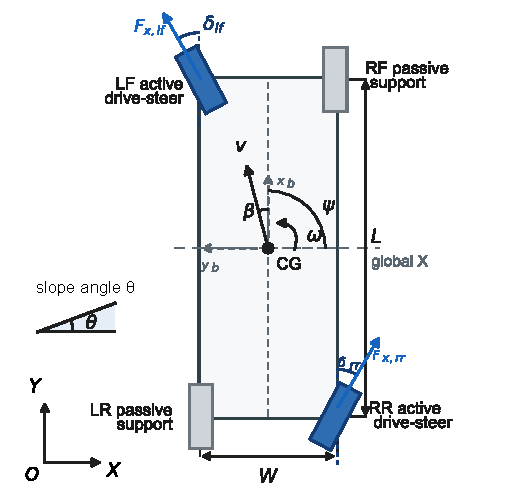
\includegraphics[width=\columnwidth]{Fig01_AGV_Configuration.pdf}
\caption{Configuration of the diagonal dual-steering-wheel AGV. The LF and RR wheels are active drive--steer wheels, while the RF and LR wheels are passive support wheels. The principal motion variables and road slope angle are indicated.}
\label{fig:agv_configuration}
\end{figure}


The considered diagonal dual-steering-wheel AGV has active drive--steer wheels at the left-front (LF) and right-rear (RR) positions, while the right-front (RF) and left-rear (LR) wheels provide passive vertical support. The normal loads of the passive wheels are retained in the load distribution and rolling resistance, whereas their lateral-force and yaw-moment contributions are neglected. The vehicle configuration and the principal motion variables are illustrated in Fig.~\ref{fig:agv_configuration}. Following the geometry-first modeling sequence used for multi-steering AGVs  \citep{Li2025FourSteeringAGV,Wan2025AGVLSTMMPC}, the steering geometry is established before the actuator, load, tire-force, and body-dynamics models.

The vehicle motion-state and control vectors are
\begin{equation}
\begin{aligned}
\bm{x}&=
\begin{bmatrix}
X & Y & \psi & v & \omega & \delta_{lf} & \delta_{rr} & \beta
\end{bmatrix}^{T},\\
\bm{u}&=
\begin{bmatrix}
F_{cmd} & \omega_{cmd}
\end{bmatrix}^{T},
\end{aligned}
\label{eq:agv_state_control}
\end{equation}
where $(X,Y)$ and $\psi$ denote the position and heading in the two-dimensional road-aligned path coordinates, $v$ is the longitudinal speed, $\omega$ is the yaw rate, $\delta_{lf}$ and $\delta_{rr}$ are the active-wheel steering angles, and $\beta$ is the vehicle sideslip angle. The longitudinal road slope angle $\theta$ is attached to the corresponding path station and enters the plant as an exogenous variable, with $\theta>0$ denoting an uphill slope along the positive direction of travel.

\subsubsection{Kinematic Model}

This study considers planar path tracking under longitudinal road slopes. The reference route is represented in a two-dimensional road-aligned coordinate chart, while the slope angle is treated as a path-dependent exogenous variable. Vertical displacement, body-pitch dynamics, road bank, and cross-slope effects are outside the present scope. Consequently, the slope angle does not directly enter the planar kinematic mapping; instead, it affects the vehicle dynamics through slope resistance, slope-dependent normal loads, and tire-force limits. The planar vehicle kinematics are therefore
\begin{equation}
\dot X=v\cos(\psi+\beta),\qquad
\dot Y=v\sin(\psi+\beta),\qquad
\dot\psi=\omega.
\label{eq:agv_kinematics}
\end{equation}
Here, the longitudinal slope is assumed to be locally aligned with the path tangent.

For curve motion, the instantaneous center of rotation (ICR) is assumed to lie on the body $y$-axis. For the smoothed speed--yaw-rate pair $(v_{icr},\omega_{icr})$, its signed radius is $R_{icr}=v_{icr}\operatorname{sgn}(\omega_{icr})/\max(|\omega_{icr}|,\varepsilon)$, where $\varepsilon=10^{-6}$. With the center of mass midway between the axles, the active-wheel steering targets are
\begin{equation}
\begin{aligned}
\delta_{lf}^{tgt}&=\arctan\!\left(\frac{L_w/2}{R_{icr}-W/2}\right),\\
\delta_{rr}^{tgt}&=-\arctan\!\left(\frac{L_w/2}{R_{icr}+W/2}\right),
\end{aligned}
\label{eq:agv_steering_geometry}
\end{equation}
where $L_w$ and $W$ are the wheelbase and track width. Both targets are set to zero when $|\omega_{cmd}|<\omega_{min}$ or $v<v_{low}$. A first-order actuator drives each $\delta_i$ toward $\delta_i^{tgt}$ with time constant $\tau_\delta$, subject to the rate bound $|\dot\delta_i|\leq\dot\delta_{max}$ and angle bound $|\delta_i|\leq\delta_{max}$.

\subsubsection{Dynamic Model}

The motor--gearbox chain limits the drive command before it reaches the wheels. For current limit $I_{max}$, torque constant $k_t$, gear ratio $n$, transmission efficiency $\eta$, and wheel radius $r$, the single-wheel force limit is $F_w^{max}=I_{max}k_t\eta n/\max(r,\varepsilon)$. The equivalent first-order current model uses $\tau_e=L_m/R_m$ and the effective current limit $I_{eff}=\min(I_{max},I_{max}^{volt})$, where $I_{max}^{volt}=\max[0,(V_{bus}-k_e\omega_m)/\max(R_m,\varepsilon)]$ and $\omega_m=|v|n/r$. The command allocation and current-to-force dynamics are
\begin{equation}
\begin{aligned}
F_{cmd}^{eff}&=\operatorname{sat}\!\left(F_{cmd},-2F_w^{max},2F_w^{max}\right),\\
F_{x,lf}^{cmd}&=F_{x,rr}^{cmd}=\frac{F_{cmd}^{eff}}{2},\\
I_i^{tgt}&=\operatorname{sat}\!\left(\frac{F_{x,i}^{cmd}r}{k_tn\eta},-I_{eff},I_{eff}\right),\\
\dot I_i&=\frac{I_i^{tgt}-I_i}{\tau_e},\qquad
F_{x,i}^{pre}=I_i\frac{k_tn\eta}{r},\quad i\in\{lf,rr\}.
\end{aligned}
\label{eq:agv_drive_actuation}
\end{equation}
The equal allocation introduces no differential drive force. The vector $\bm x$ in \eqref{eq:agv_state_control} contains only vehicle motion states. To distinguish it from the state advanced by the simulation, define the full nonlinear plant state as
\begin{equation}
\bm\zeta=
\begin{bmatrix}
\bm x^{\mathsf T}&I_{lf}&I_{rr}&\bm\zeta_f^{\mathsf T}
\end{bmatrix}^{\mathsf T},
\label{eq:full_nonlinear_state}
\end{equation}
where $\bm\zeta_f$ collects the internal states of the implemented actuator and response filters. The currents $I_{lf}$ and $I_{rr}$ are therefore first-order actuator states of the full nonlinear plant rather than elements of the vehicle motion-state vector. Their responses are retained because they provide slope-sensitive measurements for the temporal estimator. The controller introduced later uses a separate four-dimensional path-error state and does not imply that the internal plant states disappear.

The road slope enters the dynamic model through the tangential and normal components of gravity. The slope, rolling, and aerodynamic resistance terms are
\begin{equation}
\begin{aligned}
F_{slope}&=mg\sin\theta,\\
F_{roll}^{est}&=c_rmg\cos\theta,\\
F_{aero}&=\frac{1}{2}\rho_{air}C_DA\,v|v|,\\
F_{res}^{est}&=F_{roll}^{est}+F_{aero}+F_{slope}.
\end{aligned}
\label{eq:agv_slope_resistance}
\end{equation}
where $\rho_{air}$ is the air density and $C_DA$ is the product of the drag coefficient and frontal area. Thus, $mg\sin\theta$ directly changes the longitudinal force balance, whereas $mg\cos\theta$ changes the normal-load-dependent resistance and tire-force capacity. Based on the pre-clipping drive forces, the acceleration estimate, load transfers, and front--rear base loads are
\begin{equation}
\begin{aligned}
a_{long}&=\operatorname{sat}\!\left(
\frac{F_{x,lf}^{pre}+F_{x,rr}^{pre}-F_{res}^{est}}{m},-a_{max},a_{max}\right),\\
\Delta_{long}&=\frac{ma_{long}h_{cg}}{L_w},\qquad
\Delta_{lat}=\frac{m|v\omega|h_{cg}}{\max(W,\varepsilon)},\\
N_f^0&=\frac{mg\cos\theta}{2}-\Delta_{long},\qquad
N_r^0=\frac{mg\cos\theta}{2}+\Delta_{long}.
\end{aligned}
\label{eq:agv_load_transfer}
\end{equation}
Here, $N_f^0$ and $N_r^0$ denote total front- and rear-axle loads, respectively. With the lateral transfer shared equally between the two axles, the individual wheel loads before the nonnegative numerical safeguard are
\begin{equation}
\begin{aligned}
\widetilde N_{lf}&=\frac{N_f^0}{2}-\frac{\operatorname{sgn}(\omega)\Delta_{lat}}{2},&
\widetilde N_{rf}&=\frac{N_f^0}{2}+\frac{\operatorname{sgn}(\omega)\Delta_{lat}}{2},\\
\widetilde N_{lr}&=\frac{N_r^0}{2}-\frac{\operatorname{sgn}(\omega)\Delta_{lat}}{2},&
\widetilde N_{rr}&=\frac{N_r^0}{2}+\frac{\operatorname{sgn}(\omega)\Delta_{lat}}{2}.
\end{aligned}
\label{eq:agv_wheel_load_distribution}
\end{equation}
The implementation projects $\widetilde{\bm N}$ onto the nonnegative simplex with total load $mg\cos\theta$ before calculating $F_{roll}=c_r\sum_iN_i$. Because body-pitch dynamics are excluded, the model neglects the additional steady front--rear load redistribution that a pitched body could produce on a constant slope; $\Delta_{long}$ represents dynamic longitudinal transfer only.

The wheel loads constrain both lateral and longitudinal tire forces. For the two active wheels,
\begin{equation}
\begin{aligned}
\alpha_{lf}&=\delta_{lf}-\left(\beta+\frac{L_w\omega}{2\max(|v|,v_{low})}\right),\\
\alpha_{rr}&=\delta_{rr}-\left(\beta-\frac{L_w\omega}{2\max(|v|,v_{low})}\right),\\
F_{y,i}&=\operatorname{sat}\!\left(-C_{\alpha,i}\alpha_i,-\mu N_i,\mu N_i\right),\\
F_{x,i}^{allow}&=\mu N_i\sqrt{\max\!\left[1-\left(\frac{F_{y,i}}{\max(\mu N_i,\varepsilon)}\right)^2,0\right]},\\
F_{x,i}&=\operatorname{sgn}(F_{x,i}^{pre})\min\!\left(|F_{x,i}^{pre}|,F_{x,i}^{allow}\right),
\quad i\in\{lf,rr\}.
\end{aligned}
\label{eq:agv_tire_forces}
\end{equation}
For linearization, the hard saturation may be replaced by a smooth approximation. Let $\bm{R}(\delta_i)$ denote the planar rotation from wheel to body coordinates and let $\bm{r}_{lf}=[L_w/2,W/2]^T$ and $\bm{r}_{rr}=[-L_w/2,-W/2]^T$ denote the active-wheel positions. The body-frame drive resultants are
\begin{equation}
\begin{aligned}
\bm{F}^{drv}&=\sum_{i\in\{lf,rr\}}\bm{R}(\delta_i)
\begin{bmatrix}F_{x,i}\\0\end{bmatrix},\\
M_z^{drv}&=\sum_{i\in\{lf,rr\}}
\left(\bm{r}_i\times\bm{R}(\delta_i)
\begin{bmatrix}F_{x,i}\\0\end{bmatrix}\right)_z.
\end{aligned}
\label{eq:agv_drive_resultants}
\end{equation}

Finally, let $m_{eff}=m+2(I_w+I_mn^2)/r^2$ account for the reflected wheel and motor inertia. Using the resistance terms in \eqref{eq:agv_slope_resistance}, the longitudinal, yaw, and sideslip dynamics are
\begin{equation}
\begin{aligned}
\dot v&=\frac{F_x^{drv}-F_{roll}-F_{aero}-F_{slope}}
{\max(m_{eff},\varepsilon)},\\
M_z&=\frac{L_w}{2}(F_{y,lf}-F_{y,rr})+M_z^{drv}-C_{yaw}\omega,\\
\dot\omega&=\operatorname{sat}\!\left(
\frac{M_z}{\max(I_z,\varepsilon)},-\dot\omega_{max},\dot\omega_{max}\right),\\
\dot\beta&=\frac{F_{y,lf}+F_{y,rr}+F_y^{drv}}
{m_{eff}\max(|v|,v_{low}/10)}-\omega-C_{\beta}\beta.
\end{aligned}
\label{eq:agv_continuous_dynamics}
\end{equation}
At low speed, the sideslip equation is replaced by $\dot\beta=-C_{\beta}^{low}\beta$. The yaw-acceleration and sideslip-rate limits are $\dot\omega_{max}=5~\mathrm{rad/s^2}$ and $|\dot\beta|\leq10^{\circ}/\mathrm{s}$, respectively. Thus, $\theta$ does not directly change the planar kinematic mapping in \eqref{eq:agv_kinematics}; instead, $mg\sin\theta$ changes the longitudinal force balance and the $\cos\theta$-dependent wheel loads modify the available tire forces. These effects propagate through $v$, $\omega$, and $\beta$ to the path coordinates and provide the slope-sensitive onboard responses used by the temporal estimator. The parameter values that define the plant are listed in Table~\ref{tab:agv_params}; the same values are shared by data generation, LPV linearization, and closed-loop evaluation.

\begin{table}[!t]
\centering
\caption{\textbf{Physical parameters of the diagonal dual-steering-wheel AGV plant.}}
\label{tab:agv_params}
\setlength{\tabcolsep}{3pt}
\begin{tabular}{|l|l|r|}
\hline
Symbol & Description & Value \\
\hline
$m$ & Vehicle mass & $200~\mathrm{kg}$ \\
$I_z$ & Yaw moment of inertia & $16.67~\mathrm{kg\,m^2}$ \\
$L_w$ & Wheelbase & $2.0~\mathrm{m}$ \\
$W$ & Track width & $0.8~\mathrm{m}$ \\
$h_{cg}$ & Center-of-gravity height & $0.5~\mathrm{m}$ \\
\hline
$r$ & Wheel radius & $0.15~\mathrm{m}$ \\
$I_w$ & Wheel rotational inertia & $0.0135~\mathrm{kg\,m^2}$ \\
$I_m$ & Motor-rotor inertia & $1.77\times10^{-3}~\mathrm{kg\,m^2}$ \\
$k_t$ & Motor torque constant & $1.21~\mathrm{N\,m/A}$ \\
$n$ & Gear ratio & $10$ \\
$\eta$ & Transmission efficiency & $0.9$ \\
$I_{max}$ & Per-motor current limit & $9.0~\mathrm{A}$ \\
\hline
$\tau_\delta$ & Steering time constant & $0.08~\mathrm{s}$ \\
$\delta_{max}$ & Steering-angle limit & $90^{\circ}$ \\
$\dot\delta_{max}$ & Steering-rate limit & $30^{\circ}/\mathrm{s}$ \\
$a_{max}$ & Longitudinal-acceleration bound & $1.0~\mathrm{m/s^2}$ \\
\hline
$C_{\alpha}$ & Cornering stiffness (each active wheel) & $3000~\mathrm{N/rad}$ \\
$\mu$ & Tire--road friction coefficient & $0.8$ \\
$c_r$ & Rolling-resistance coefficient & $0.015$ \\
$\rho_{air}$ & Air density & $1.225~\mathrm{kg/m^3}$ \\
$C_DA$ & Drag-area product & $0.5~\mathrm{m^2}$ \\
$C_{yaw}$ & Yaw damping coefficient & $250~\mathrm{N\,m\,s/rad}$ \\
$C_{\beta}$, $C_{\beta}^{low}$ & Sideslip damping (normal, low speed) & $0$, $1.0~\mathrm{s^{-1}}$ \\
\hline
\end{tabular}
\end{table}


\subsection{Slope-Aware Path-Tracking Objective and Problem Formulation}

The objective of this work is constrained path tracking under longitudinal
slope variations, rather than slope estimation as an end in itself; slope coupling has likewise motivated dedicated adaptive tracking designs for multi-wheel-drive platforms \citep{Zhang2025CoupledSlope4WID}. The
tracking error is defined as
$\bm e_k=[e_{y,k},e_{\psi,k},e_{v,k},e_{\omega,k}^{\mathrm{trk}}]^{T}$, which
collects the lateral, heading, longitudinal-speed, and yaw-rate errors. The
superscript distinguishes $e_{\omega}^{\mathrm{trk}}$ from the kinematic
yaw-consistency feature introduced in
Section~\ref{sec:proposed_framework}. The control problem is stated in the
general form
\begin{equation}
\begin{aligned}
\min_{\{\bm u_k\}}\quad &J_{\mathrm{track}}(\bm e,\Delta\bm u)\\
\mathrm{s.t.}\quad
&\bm\zeta_{k+1}=\mathcal F_{T_s}(\bm\zeta_k,\bm u_k,\theta_k),\\
&\bm u_k\in\mathcal U,\qquad
\Delta\bm u_k\in\Delta\mathcal U,
\end{aligned}
\label{eq:slope_aware_tracking_objective}
\end{equation}
where $J_{\mathrm{track}}$ is the finite-horizon path-tracking cost,
$\Delta\bm u_k=\bm u_k-\bm u_{k-1}$ is the control increment,
$\mathcal F_{T_s}(\cdot)$ is the one-step AGV state-transition map over
sampling interval $T_s$, and $\mathcal U$ and $\Delta\mathcal U$ are the
admissible input and input-increment sets. The full cost and constraints are
specified in Section~\ref{sec:model_lpv_mpc}. Within
this problem, the slope angle is a control-relevant variable rather than an
isolated geometric quantity. It changes the longitudinal force balance
through $mg\sin\theta_k$ in \eqref{eq:agv_slope_resistance} and modifies the
available tire forces through the $\cos\theta_k$-dependent wheel loads in
\eqref{eq:agv_tire_forces}. Scheduling the controller with an inaccurate
slope therefore makes the prediction model inconsistent with the plant and
degrades closed-loop tracking
performance~\citep{Sato2013InexactScheduling,Metzler2021PredictionFidelity}.

A direct route to $\theta_k$ is inertial sensing. However, IMU-derived slope
estimates can be biased by transient longitudinal acceleration, body-pitch
excitation, road-induced vibration, and low-cost sensor
noise~\citep{Liu2023RoadSlopeAAIMM}. Model-based observers that fuse
inertial and drivetrain information also remain sensitive to
vehicle-parameter mismatch and load
variation~\citep{Gao2024RoadSlopeHDV}. The controller is therefore assumed
to have access to neither the true slope nor a reliable instantaneous
inertial measurement. Instead, the current slope is inferred from a fixed
window of onboard responses available at the sampling instant,
\begin{equation}
\mathcal H_k=\left(\bm s_{k-N_h+1},\bm s_{k-N_h+2},\ldots,\bm s_k\right),
\qquad
\hat\theta_k^{\mathrm{hist}}=f_{\phi}(\mathcal H_k),
\label{eq:slope_estimation_objective}
\end{equation}
Here, $\mathcal H_k$ is the ordered $N_h$-sample history ending at $k$, and
$\bm s_k$ collects measured or recursively derived proprioceptive quantities.
The learned map $f_{\phi}(\cdot)$, parameterized by $\phi$, produces the
history-based slope estimate $\hat\theta_k^{\mathrm{hist}}$. The true slope
and any direct pitch-based slope measurement are
excluded from the estimator input, and no sample later than the current
instant $k$ is used. The window length $N_h$ balances the observability of
slope-induced responses against the dilution of slope-transition
information. Its numerical value and the underlying response-time
calculation are reported with the experimental settings.

These considerations reduce slope-aware tracking to four coupled
requirements: a lightweight history-based temporal estimator,
dynamics-informed feature and multi-scale lag construction,
uncertainty-adaptive fusion of the history-based estimate and the qualified observer estimate, and
synchronized incorporation of the fused slope into all slope-dependent
LPV-MPC updates. Section~\ref{sec:proposed_framework} develops these
components in turn to support the tracking objective in
\eqref{eq:slope_aware_tracking_objective}.

\begin{figure*}[!tbp]
\centering
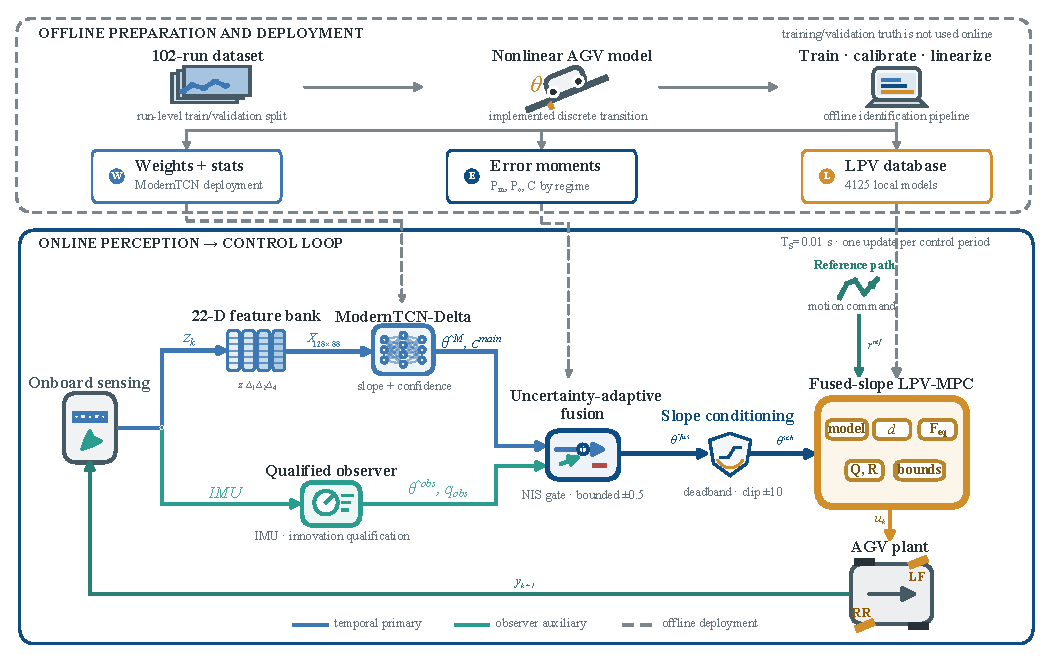
\includegraphics[width=\textwidth]{Fig02_Slope_Aware_Perception_Control_Framework.pdf}
\caption{Overall slope-aware perception-and-control framework. Offline preparation uses the 102-run dataset and nonlinear AGV model to deploy the ModernTCN weights and normalization statistics, fusion-error moments, and 4125-model LPV database. Online, onboard sensing drives the 22-D feature-bank/ModernTCN-Delta primary branch and the qualified observer auxiliary branch in parallel. Their uncertainty-adaptive fusion is conditioned to form $\theta_k^{\mathrm{sch}}$, which synchronously updates the LPV-MPC model, disturbance and equivalent-force terms, weights, and constraints before control of the nonlinear AGV plant. Solid blue and green paths denote the temporal-primary and observer-auxiliary signals, respectively; dashed gray paths denote offline deployment.}
\label{fig:overall_framework}
\end{figure*}

\section{Slope-Aware Temporal Perception and LPV-MPC Framework}
\label{sec:proposed_framework}

The formulation in Section~\ref{sec:agv_slope_estimation} creates a perception-to-control chain rather than four independent additions. The first problem is to infer a control-relevant slope from onboard histories without using a direct slope channel. The second is to expose both the absolute operating state and the short slope-sensitive changes that an instantaneous input can obscure. The third is to reconcile the complementary but condition-dependent information supplied by the temporal estimator and the qualified observer. The final problem is to inject one physically consistent slope signal into every slope-dependent LPV-MPC update. Accordingly, the proposed framework proceeds from a lightweight ModernTCN estimator, through dynamics-informed feature construction and multi-scale time-lag differences, to adaptive slope fusion and synchronized LPV-MPC scheduling. Here, time-lag enhancement denotes the construction of temporal-difference channels between the current normalized feature vector and its lagged counterparts at multiple offsets. Figure~\ref{fig:overall_framework} summarizes this pipeline and its interfaces: onboard measurement histories feed the temporal-perception branch and the qualified observer branch in parallel, a single conditioned fused slope $\theta_k^{\mathrm{sch}}$ crosses the perception-to-control boundary, and every slope-dependent element of the LPV-MPC update is scheduled from this signal synchronously.

\subsection{Lightweight ModernTCN-Based Slope Estimator}

To implement the history-to-slope mapping in \eqref{eq:slope_estimation_objective}, a lightweight task-specific estimator is developed from the temporal modeling principles of ModernTCN~\citep{Luo2024ModernTCN}. The estimator retains large-kernel depthwise temporal convolution, pointwise channel mixing, and residual learning, while removing the full patch-based and multi-stage hierarchy of the original general-purpose architecture. This reduction gives a fixed-window network that can be exported through ONNX and executed within the MATLAB/Simulink closed loop.

Let the network input be written generically as
\begin{equation}
\mathbf Z_k\in\mathbb R^{N_h\times F},
\label{eq:generic_moderntcn_input}
\end{equation}
where its physical channels and temporal augmentation are specified in the following two subsections. A pointwise stem first projects the input to a latent channel space,
\begin{equation}
\mathbf H_k^{(0)}=\sigma\!\left[
\operatorname{BN}\!\left(
\operatorname{Conv}_{1\times1}(\mathbf Z_k^{\mathsf T})
\right)\right],
\label{eq:moderntcn_stem}
\end{equation}
where $\mathbf H_k^{(0)}\in\mathbb R^{C\times N_h}$, $C=64$, $\operatorname{BN}(\cdot)$ denotes batch normalization, and $\sigma(\cdot)$ is the ReLU activation. Five stride-one residual temporal blocks are then applied. The $\ell$-th block is
\begin{align}
\mathbf U_k^{(\ell)}
 &=\operatorname{DWConv}_{K}\!\left(\mathbf H_k^{(\ell)}\right),\nonumber\\
\mathbf V_k^{(\ell)}
 &=\operatorname{PW}_{2}^{(\ell)}\!\left\{
\sigma\!\left[\operatorname{PW}_{1}^{(\ell)}
\!\left(\sigma\!\left[\operatorname{BN}
(\mathbf U_k^{(\ell)})\right]\right)\right]\right\},\nonumber\\
\mathbf H_k^{(\ell+1)}
 &=\mathbf H_k^{(\ell)}
 +\gamma_{\ell}\operatorname{BN}\!\left(\mathbf V_k^{(\ell)}\right),
\label{eq:moderntcn_small_block}
\end{align}
where $\operatorname{DWConv}_{K}$ is a depthwise temporal convolution with $K=31$, the two pointwise convolutions use an expansion ratio of two, and $\gamma_{\ell}$ is a learnable residual scale. The five large-kernel blocks provide a nominal receptive field of 151 samples, thereby covering the implemented historical window.

The final sequence is summarized by its last, mean, and maximum latent responses. Window-level statistics of the normalized input are added to retain low-order information about each channel:
\begin{equation}
\begin{aligned}
\mathbf h_k={}&\left[
\mathbf H_{k,:,N_h}^{(5)};
\operatorname{mean}_{t}\mathbf H_{k,:,t}^{(5)};
\operatorname{max}_{t}\mathbf H_{k,:,t}^{(5)};
q(\mathbf Z_k)\right],\\
\hat{\theta}^{\mathrm{raw}}_k
 ={}&\mathbf w_{\theta}^{\mathsf T}\mathbf h_k+b_{\theta},
\end{aligned}
\label{eq:moderntcn_readout}
\end{equation}
where $q(\mathbf Z_k)$ concatenates the current value, mean, standard deviation, maximum, and minimum of each input channel. Although same padding is used inside the fixed window, $\mathbf Z_k$ terminates at the current sample and contains no measurement later than $k$. The deployed estimator is therefore a history-only online mapping; it is not described as a strictly causal convolutional backbone. Before fusion, the raw regression output is processed by a causal deployment interface, which applies first-order temporal smoothing, the configured physical magnitude and rate limits, and the MPC-side deadband. The resulting control-facing ModernTCN-Delta estimate is denoted by $\hat{\theta}^{\mathrm{MTCN}}_k$ in the remainder of this section. This distinction prevents the network readout from being conflated with the stateful signal actually consumed by the fusion module.

The shared representation additionally feeds two auxiliary classification heads,
\begin{equation}
\begin{aligned}
\hat{\mathbf p}^{\mathrm{main}}_k
&=\operatorname{softmax}\!\left(g_{\mathrm{main}}(\mathbf h_k)\right),\\
\hat{\mathbf p}^{\mathrm{turn}}_k
&=\operatorname{softmax}\!\left(g_{\mathrm{turn}}(\mathbf h_k)\right),
\end{aligned}
\label{eq:slope_auxiliary_outputs}
\end{equation}
which identify the main operating condition and steering direction. Both heads are auxiliary to slope regression and are not evaluated as independent perception contributions. The steering-direction output is retained for representation learning and diagnostics; only $c_k^{\mathrm{main}}=\max(\hat{\mathbf p}^{\mathrm{main}}_k)$ enters the deployed interface, where it calibrates the ModernTCN uncertainty used by the fusion weight. Neither predicted label directly schedules the controller or acts as a hard switching predicate. The training objective is
\begin{equation}
\mathcal L=
\lambda_{\theta}\mathcal L_{\theta}
+\mathcal L_{\mathrm{main}}
+\lambda_{\mathrm{turn}}\mathcal L_{\mathrm{turn}}
+\mathcal R_{\theta},
\label{eq:slope_estimator_loss}
\end{equation}
where $\mathcal R_{\theta}$ collects the flat-road and bounded-error slope penalties. Table~\ref{tab:moderntcn_variant_comparison} distinguishes the implemented network from the complete ModernTCN architecture.

\begin{table*}[!tbp]
\centering
\caption{\textbf{Structural distinction between the original ModernTCN and the lightweight task-specific estimator.}}
\label{tab:moderntcn_variant_comparison}
\setlength{\tabcolsep}{3pt}
\begin{tabular}{|p{0.20\textwidth}|p{0.35\textwidth}|p{0.37\textwidth}|}
\hline
Component & Original ModernTCN~\citep{Luo2024ModernTCN} & Lightweight task-specific estimator used in this work \\
\hline
Input embedding & Variable-independent patch embedding with an explicit variable dimension & Joint $1\times1$ channel projection of the fixed historical input \\
Temporal modeling & Large- and small-kernel depthwise convolutions with structural re-parameterization & One large-kernel depthwise convolution ($K=31$) in each residual block \\
Feature mixing & Decoupled grouped ConvFFN modules for within- and cross-variable interaction & Two standard pointwise convolutions with an expansion ratio of two \\
Backbone hierarchy & Patch tokens and a multi-stage representation hierarchy & Five repeated stride-one residual blocks with 64 latent channels \\
Readout and deployment & Task-dependent pipelines for general time-series analysis & Last/mean/max latent pooling plus input statistics, slope and auxiliary heads, and ONNX deployment in MATLAB/Simulink \\
\hline
\end{tabular}
\end{table*}

\subsection{Dynamics-Informed 22-D Proprioceptive Feature Construction}

The temporal architecture alone does not determine whether the input contains identifiable slope information. The AGV model shows that slope first changes longitudinal resistance and available tire forces, after which its effects appear jointly in speed, acceleration, drive effort, wheel asymmetry, and yaw--steering consistency. The estimator input is therefore restricted to online onboard measurements and recursively computed response variables that represent these complementary mechanisms, consistent with longitudinal-dynamics-based estimation from standard IMU and CAN-bus signals \citep{Jensen2022MassGradeIMUCAN}. The resulting fixed feature vector is
\begin{equation}
\begin{aligned}
\mathbf{s}_k=\big[&
\omega_{g},I_{lf},I_{rr},\omega_{w,lf},\omega_{w,rr},
\delta_{lf},\delta_{rr},\\
&\hat v,\dot{\hat v},\Delta\omega_w,I_{\Sigma},
\Delta I,\Delta I_{|\cdot|},\\
&\hat\kappa,a_I,\dot{\hat v}_{\mathrm{LP}},a_{x,w},
I_{\mathrm{drv}},I_a,\Lambda,a_{\mathrm{HP}},\varepsilon_{\omega}^{\mathrm{kin}}
\big]_k^{\mathsf T}\in\mathbb R^{22}.
\end{aligned}
\label{eq:feature_vector_22d}
\end{equation}

Here, $\omega_g$ is the measured yaw rate; $I_{lf}$ and $I_{rr}$ are the active-wheel motor currents; $\omega_{w,lf}$ and $\omega_{w,rr}$ are the corresponding wheel speeds; and $\delta_{lf}$ and $\delta_{rr}$ are the steering angles. The wheel-speed-derived motion responses are updated recursively as
\begin{align}
\hat v_k&=\frac{r}{2}\left(\omega_{w,lf,k}+\omega_{w,rr,k}\right),\nonumber\\
a_{x,w,k}&=\frac{\hat v_k-\hat v_{k-1}}{T_s},\nonumber\\
\dot{\hat v}_k&=\alpha_d a_{x,w,k}
+(1-\alpha_d)\dot{\hat v}_{k-1},\nonumber\\
\dot{\hat v}_{\mathrm{LP},k}
&=\alpha_{\mathrm{LP}}\dot{\hat v}_k
+(1-\alpha_{\mathrm{LP}})\dot{\hat v}_{\mathrm{LP},k-1},\nonumber\\
a_{\mathrm{HP},k}&=a_{x,w,k}-\dot{\hat v}_{\mathrm{LP},k},
\label{eq:kinematic_feature_channels}
\end{align}
where $\alpha_d=T_s/(\tau_d+T_s)$ and $\alpha_{\mathrm{LP}}=T_s/(\tau_{\mathrm{LP}}+T_s)$. The raw, filtered, and high-pass terms retain rapid wheel-speed changes, the persistent acceleration trend, and short longitudinal transients, respectively.

At the low operating speeds considered here, $\hat v$ is used only as a wheel-speed-derived motion proxy. It does not correct for steering projection or longitudinal slip and is therefore not interpreted as an exact vehicle speed during sharp steering or tire slip. The bilateral drive responses are
\begin{align}
\Delta\omega_{w,k}&=\left|\omega_{w,lf,k}-\omega_{w,rr,k}\right|,\nonumber\\
I_{\Sigma,k}&=|I_{lf,k}|+|I_{rr,k}|,\qquad
\Delta I_k=I_{lf,k}-I_{rr,k},\nonumber\\
\Delta I_{|\cdot|,k}&=|I_{lf,k}|-|I_{rr,k}|,\qquad
I_{\mathrm{drv},k}=I_{lf,k}+I_{rr,k},
\label{eq:drive_asymmetry_channels}
\end{align}
which distinguish total traction demand from unequal wheel loading and turning-related allocation. The remaining consistency variables are
\begin{align}
\hat\kappa_k&=\frac{\tan\delta_{lf,k}-\tan\delta_{rr,k}}{L_w},\nonumber\\
a_{I,k}&=\frac{\dot{\hat v}_k}{\max(I_{\Sigma,k},I_{\min})},\qquad
I_{a,k}=\frac{I_{\Sigma,k}}
{\max(|\dot{\hat v}_{\mathrm{LP},k}|,a_{\min})},\nonumber\\
\Lambda_k&=
\frac{I_{\mathrm{drv},k}-\mu_{I,\mathrm{tr}}}{\max(\sigma_{I,\mathrm{tr}},\epsilon_N)}
-\frac{\dot{\hat v}_{\mathrm{LP},k}-\mu_{a,\mathrm{tr}}}{\max(\sigma_{a,\mathrm{tr}},\epsilon_N)},\nonumber\\
\varepsilon_{\omega,k}^{\mathrm{kin}}&=\omega_{g,k}-\hat v_k\hat\kappa_k .
\label{eq:load_consistency_channels}
\end{align}
The protected denominators $I_{\min}=0.1$ and $a_{\min}=0.05$ prevent singular behavior at low current or acceleration. The statistics $(\mu_{I,\mathrm{tr}},\sigma_{I,\mathrm{tr}})$ and $(\mu_{a,\mathrm{tr}},\sigma_{a,\mathrm{tr}})$ are fitted on the training split, and $\epsilon_N>0$ protects the standardization. Thus, $\Lambda_k$ combines two separately standardized quantities and is dimensionless; it is interpreted as an empirical drive--response co-variation feature rather than as a physical force. The denominator $L_w$ in $\hat\kappa_k$ follows the front--rear steering geometry in \eqref{eq:agv_steering_geometry}; the quantity remains a low-speed curvature proxy because slip and passive-wheel kinematics are omitted. Finally, $\varepsilon_{\omega,k}^{\mathrm{kin}}$ expresses yaw inconsistency and is distinct from the MPC tracking error $e_{\omega,k}^{\mathrm{trk}}$. The complete 22-channel input contract assembled from these mechanisms is listed in Table~\ref{tab:feature_contract_22d}.

\begin{table*}[!tbp]
\centering
\caption{\textbf{Dynamics-informed 22-dimensional proprioceptive feature set.}}
\label{tab:feature_contract_22d}
\setlength{\tabcolsep}{3pt}
\begin{tabular}{|>{\raggedright\arraybackslash}p{0.16\textwidth}|>{\centering\arraybackslash}p{0.05\textwidth}|>{\raggedright\arraybackslash}p{0.39\textwidth}|>{\raggedright\arraybackslash}p{0.28\textwidth}|}
\hline
Feature group & Dim. & Implemented channels & Primary information represented \\
\hline
Raw onboard sensing & 7 & \texttt{gyro\_z}, \texttt{I\_lf}, \texttt{I\_rr}, \texttt{omega\_wheel\_lf}, \texttt{omega\_wheel\_rr}, \texttt{delta\_lf}, \texttt{delta\_rr} & Measured yaw, drive effort, wheel motion, and steering state \\
Kinematic and multi-band response & 5 & \texttt{v\_hat}, \texttt{dv\_hat\_dt}, \texttt{dv\_hat\_dt\_lp}, \texttt{accel\_x\_wheel}, \texttt{a\_hp} & Current speed, persistent acceleration trend, and rapid longitudinal transients \\
Drive asymmetry and allocation & 5 & \texttt{ws\_imbalance}, \texttt{I\_sum}, \texttt{I\_diff\_signed}, \texttt{I\_diff\_abs}, \texttt{I\_drive\_signed} & Total traction demand and unequal active-wheel response \\
Load and kinematic consistency proxies & 5 & \texttt{kappa\_proxy}, \texttt{accel\_per\_current}, \texttt{current\_per\_accel}, \texttt{drive\_load\_proxy}, \texttt{yaw\_consistency\_error} & Steering curvature, drive--acceleration coupling, and yaw inconsistency \\
\hline
\end{tabular}
\end{table*}

The feature set excludes global pose, unmeasured sideslip and wheel normal loads, the true road slope, and direct pitch- or slope-measurement channels. The yaw-rate gyroscope remains because it measures rotational vehicle response rather than slope. Thus, the network must infer slope from the coupled response pattern of the AGV instead of learning an identity mapping from a direct slope measurement.

\subsection{Multi-Scale Time-Lag Difference Representation and Historical Window Assembly}

Even with the 22-D feature set, a single sample is ambiguous because similar current and acceleration levels can be produced by slope resistance, a traction or braking command, or a steering transition. Sequence models over onboard response histories have proven effective for related road-condition identification tasks \citep{Liang2022LSTMRoadID}. Temporal differences are therefore constructed after train-set normalization,
\begin{equation}
\mathbf z_k=\mathcal N(\mathbf s_k)
=\frac{\mathbf s_k-\boldsymbol\mu_{\mathrm{tr}}}
{\boldsymbol\sigma_{\mathrm{tr}}},
\label{eq:feature_train_normalization}
\end{equation}
where $\boldsymbol\mu_{\mathrm{tr}}$ and $\boldsymbol\sigma_{\mathrm{tr}}$ are fitted only on the training split. For a lag $\ell$, the normalized delta channel is
\begin{equation}
\Delta_{\ell}\mathbf z_k=
\operatorname{clip}\!\left(
\mathbf z_k-\mathbf z_{k-\ell},-c_{\Delta},c_{\Delta}
\right),\qquad \ell\in\{1,2,4\},
\label{eq:multiscale_delta_lag}
\end{equation}
with $c_{\Delta}=5$. At $T_s=0.01$ s, the three offsets represent 10, 20, and 40 ms response changes. The augmented vector is
\begin{equation}
\widetilde{\mathbf z}_k=
\begin{bmatrix}
\mathbf z_k^{\mathsf T}&
(\Delta_1\mathbf z_k)^{\mathsf T}&
(\Delta_2\mathbf z_k)^{\mathsf T}&
(\Delta_4\mathbf z_k)^{\mathsf T}
\end{bmatrix}^{\mathsf T}
\in\mathbb R^{88}.
\label{eq:delta_bank_124}
\end{equation}

The augmented representation in \eqref{eq:delta_bank_124} is referred to as the delta bank. The current normalized state retains the absolute operating condition, whereas the three difference blocks expose increasingly wider local changes. Calculating the differences after normalization prevents the wheel-speed and current scales from dominating the augmentation, and clipping limits isolated transients. The lag set was configured through a staged representation study: single offsets from $\{1,2,4,8,16,32,64\}$ were first screened, after which the short offsets $\{1,2,4\}$ were carried forward. Raw input, a single-difference branch, multi-lag state stacking, the three-branch delta bank, and mixed lag--delta inputs were then compared under the same estimator and synchronized deployment interface. The deployed delta bank is evaluated through the matched-seed offline comparison in Section~\ref{subsec:offline_delta_lag_evaluation} and the closed-loop slope-estimation comparison in Section~\ref{subsec:closed_loop_estimator_accuracy}.

The 88-dimensional vectors are placed in chronological order,
\begin{equation}
\mathbf Z_k=
\begin{bmatrix}
\widetilde{\mathbf z}_{k-N_h+1}^{\mathsf T}\\
\widetilde{\mathbf z}_{k-N_h+2}^{\mathsf T}\\
\vdots\\
\widetilde{\mathbf z}_{k}^{\mathsf T}
\end{bmatrix}
\in\mathbb R^{N_h\times88},\qquad N_h=128.
\label{eq:historical_input_128x88}
\end{equation}
At the 0.01s sampling interval, the implemented window covers 1.28 s. Its length is fixed from the characteristic response time over which slope-induced resistance produces an observable change in the onboard responses at the representative speed, slope, and effective inertia of the present AGV; the corresponding parameter calculation is given in the experimental setup. For unavailable lagged samples at the beginning of a window, the first normalized sample is used for edge padding, which makes the corresponding differences zero. The same normalization, padding, endpoint labeling, and channel order are used during dataset construction, validation, ONNX export, and online inference.

\subsection{Uncertainty-Adaptive Slope Fusion with the Qualified Observer}
\label{sec:adaptive_slope_fusion}

ModernTCN-Delta and the qualified observer provide complementary information
for road slope perception. ModernTCN-Delta remains the primary source because
it estimates slope from history-based vehicle responses, whereas the qualified
observer contributes an auxiliary inertial observation. The observer follows
the low-dynamic MEMS-IMU estimation structure of
\citep{Chen2024RobustAttitude} and adopts innovation-based adaptive-noise
modulation in the spirit of \citep{Guo2022SageHusaAKF}. In the present
implementation, the observer receives the bias-compensated six-axis packet
$[\tilde f_x,\tilde f_y,\tilde f_z,\tilde g_x,\tilde g_y,\tilde g_z]^{T}$ at
$T_s=0.01$~s and provides a slope-related output for the fusion interface.

The observer propagates a pitch-related state and gyroscope-bias state from the
angular-rate measurements and updates them with the accelerometer-derived
gravity observation. Its innovation is
\begin{equation}
\bm r_k^{a}=\bm z_k^{a}-h_{\mathrm{obs}}(\bm x_k^{-}),
\qquad
\bm x_k^{-}=f_{\mathrm{obs}}(\bm x_{k-1},
\tilde{\bm\omega}_k),
\label{eq:qualified_observer_prediction}
\end{equation}
where $\bm z_k^{a}=[\tilde f_x,\tilde f_y,\tilde f_z]^{T}$, and
$f_{\mathrm{obs}}(\cdot)$ and $h_{\mathrm{obs}}(\cdot)$ denote the
bias-compensated propagation and gravity-observation maps. The observation
covariance is modulated by normalized acceleration-norm, vibration, and
innovation scores,
\begin{equation}
\begin{aligned}
\bm R_k&=\bm R_0\,
\operatorname{clip}\!\left(m_k,1,m_{\max}\right),\\
m_k&=\mathcal F\!\left(
w_n s_k^{n},w_v s_k^{v},w_{\nu}s_k^{\nu}\right),
\end{aligned}
\label{eq:qualified_observer_adaptation}
\end{equation}
where $(w_n,w_v,w_{\nu})=(0.50,0.15,0.35)$, the vibration persistence factor
is $0.95$, and $m_{\max}=60$. The deployed normalization scales are
$0.2g$, $0.35$~rad/s, and $4^{\circ}$ for the acceleration norm, angular
rate, and innovation, respectively. The initial pitch standard deviation is
$2^{\circ}$, the initial gyroscope-bias standard deviation is
$0.01$~rad/s, the gyroscope-noise standard deviation is $0.002$~rad/s, the
bias random-walk standard deviation is $5\times10^{-5}$~rad/s, and the
accelerometer-derived pitch standard deviation is $1.25^{\circ}$. The
resulting observer state is converted to the slope interface
\begin{equation}
\hat\theta_k^{\mathrm{obs}}=\mathcal G_{\theta}(\bm x_k^{\mathrm{obs}}),
\label{eq:qualified_observer_grade_output}
\end{equation}
where $\mathcal G_{\theta}(\cdot)$ denotes the road-aligned slope conversion.

Fusion uncertainty is calibrated offline from the training and validation
runs. Ground-truth slope is used only for this calibration and is absent from
the deployed interface. The calibration stores regime-dependent total error
moments for ModernTCN-Delta and the qualified observer, including their
cross-error moment. At runtime, the ModernTCN confidence and the observer
quality score adjust these moments before the innovation test. With
\[
\nu_k=\hat\theta_k^{\mathrm{obs}}-\hat\theta_k^{\mathrm{MTCN}},
\]
the innovation variance, NIS, and raw gain are
\begin{equation}
\begin{aligned}
S_k&=\max(P_{\mathrm{M},k}+P_{\mathrm{O},k}-2C_k,S_{\min}),\\
\mathrm{NIS}_k&=\nu_k^2/S_k,\qquad
K_k^{\mathrm{raw}}=(P_{\mathrm{M},k}-C_k)/S_k .
\end{aligned}
\label{eq:adaptive_observer_gain}
\end{equation}
The effective gain is
\begin{equation}
\begin{aligned}
K_k^{\mathrm{eff}}
&=\eta_k\operatorname{clip}(K_k^{\mathrm{raw}},0,1),\\
\eta_k
&=\begin{cases}
1, & \mathrm{NIS}_k\leq 9,\\
\sqrt{9/\mathrm{NIS}_k}, & 9<\mathrm{NIS}_k\leq 25,\\
0, & \mathrm{NIS}_k>25.
\end{cases}
\end{aligned}
\label{eq:innovation_conditioned_observer_gain}
\end{equation}
The selected configuration uses $K_{\max}=1.0$, a helpfulness threshold of
0.6, slope-entry and slope-exit thresholds of $0.5^{\circ}$ and
$0.3^{\circ}$, respectively, a minimum innovation of $0.25^{\circ}$, and an
innovation rejection gate of $2^{\circ}$. Equation~\eqref{eq:innovation_conditioned_observer_gain}
defines the gain within an eligible correction state; otherwise, the exact
identity fallback is used.

The target correction and its causal update are
\begin{align}
\delta\theta_k^{\star}
&=\operatorname{clip}\!\left[
K_k^{\mathrm{eff}}\nu_k,-0.5^{\circ},0.5^{\circ}\right],\nonumber\\
\delta\theta_k
&=\delta\theta_{k-1}
+\operatorname{clip}\!\left[
\delta\theta_k^{\star}-\delta\theta_{k-1},
-5^{\circ}\mathrm{s}^{-1}T_s,5^{\circ}\mathrm{s}^{-1}T_s\right],\nonumber\\
\hat\theta_k^{\mathrm{fus}}
&=\hat\theta_k^{\mathrm{MTCN}}+\delta\theta_k .
\label{eq:adaptive_slope_fusion}
\end{align}
If the temporal estimate is not ready, the qualified observer is unavailable,
the helpfulness or slope-hysteresis condition is not satisfied, the innovation
is below the minimum activation level or exceeds $2^{\circ}$, or
$\mathrm{NIS}_k>25$, the exact identity fallback is applied:
$\hat\theta_k^{\mathrm{fus}}=\hat\theta_k^{\mathrm{MTCN}}$ and
$\delta\theta_k=0$. Before entering the controller, the fused slope is
processed by the $1.3^{\circ}$ deadband, clipped to
$[-10^{\circ},10^{\circ}]$, and passed through the causal scheduling filter.
The resulting $\theta_k^{\mathrm{sch}}$ is the single slope signal supplied to
the LPV prediction model, measured-disturbance channel, slope feedforward,
scheduled weights, and constraints. It is defined by
\begin{equation}
\theta_k^{\mathrm{sch}}=\mathcal F_{\rho}\!\left(\theta_k^{\mathrm{guard}}\right),
\label{eq:fused_slope_conditioning}
\end{equation}
where $\mathcal F_{\rho}(\cdot)$ denotes the unchanged causal scheduling
filter.

Algorithm~\ref{alg:online_slope_fusion} summarizes the online execution order.
\begin{algorithm}[!t]
\caption{Online slope fusion assisted by the qualified observer}
\label{alg:online_slope_fusion}
\begin{algorithmic}[1]
\Require ModernTCN-Delta estimate and confidence; current six-axis inertial packet
\Ensure scheduled slope $\theta_k^{\mathrm{sch}}$
\State Propagate and update the qualified observer using
\eqref{eq:qualified_observer_prediction}--\eqref{eq:qualified_observer_adaptation}
\State Compute $\hat\theta_k^{\mathrm{obs}}$, $\nu_k$, $\mathrm{NIS}_k$, and
$K_k^{\mathrm{eff}}$
\If{any readiness, helpfulness, slope, or innovation-consistency gate fails}
    \State Apply exact identity fallback
\Else
    \State Apply the bounded, rate-limited correction in
    \eqref{eq:adaptive_slope_fusion}
\EndIf
\State Apply the amplitude guard and causal scheduling filter
\State \Return $\theta_k^{\mathrm{sch}}$
\end{algorithmic}
\end{algorithm}

\subsection{Fusion-Based Slope-Scheduled Discrete LPV-MPC}
\label{sec:model_lpv_mpc}

The fusion module becomes control-relevant only when its output modifies the prediction model and optimization problem consistently. The nonlinear plant is therefore converted to a discrete LPV prediction model using the same actuator update and numerical transition as the closed-loop simulation, after which the conditioned slope in \eqref{eq:fused_slope_conditioning} synchronously schedules the model, measured-disturbance path, feedforward term, weights, and bounds, following the established LPV-MPC practice of offline model construction with online scheduled updates \citep{Uchihori2021AUVLPVMPC}.

\subsubsection{Discrete Path-Error Model}

The controller state, input, and measured slope disturbance are
\begin{equation}
\begin{aligned}
\bm{x}^{e}_k
&=\begin{bmatrix}e_{y,k}&e_{\psi,k}&e_{v,k}&e_{\omega,k}^{\mathrm{trk}}\end{bmatrix}^{T},\\
\bm{u}_k
&=\begin{bmatrix}F_{cmd,k}&\omega_{cmd,k}\end{bmatrix}^{T},
\qquad d_k=\theta^{\mathrm{sch}}_k .
\end{aligned}
\label{eq:discrete_error_state}
\end{equation}
Let $\Phi_{T_s}$ denote the implemented one-step transition of the full state $\bm\zeta$ in \eqref{eq:full_nonlinear_state}, including steering-rate and steering-angle saturation, midpoint steering values, fourth-order Runge--Kutta integration, angle wrapping, non-negative-speed protection, and sideslip limiting. The lifting map $\mathcal L_e(\bm x^e;\bm r^{ref},\bar{\bm\zeta}_{int})$ reconstructs the absolute motion state from the path-error coordinates and the local reference pose, speed, and yaw rate, and inserts the steering, sideslip, current, and filter states $\bar{\bm\zeta}_{int}$ associated with the local operating point. Conversely, $\bm q(\bm\zeta;\bm r^{ref})$ maps the propagated absolute state back to the four path errors. The implemented reduced transition is therefore
\begin{equation}
\bm g(\bm x^e,\bm u,\theta)
=\bm q\!\left(
\Phi_{T_s}\!\left[
\mathcal L_e(\bm x^e;\bm r^{ref},\bar{\bm\zeta}_{int}),
\bm u,\theta\right],\bm r^{ref,+}
\right).
\label{eq:implemented_error_transition}
\end{equation}
During nonlinear simulation, all components of $\bm\zeta$ are advanced. During offline database construction, the reduced four-state model fixes the unrepresented internal states at their local operating values before finite differentiation. This makes the reduction and its approximation explicit. Define the operating-point deviations
\begin{equation}
\widetilde{\bm x}^{e}_k=\bm x^e_k-\bar{\bm x}^{e},\qquad
\widetilde{\bm u}_k=\bm u_k-\bar{\bm u},\qquad
\widetilde\theta_k=\theta_k-\bar\theta,
\label{eq:operating_point_deviations}
\end{equation}
whereas the control increment is reserved for the adjacent-sample difference $\Delta\bm u_k=\bm u_k-\bm u_{k-1}$. The local deviation model is
\begin{align}
\widetilde{\bm{x}}^{e}_{k+1}
&=A_d(\boldsymbol\varrho_k)\widetilde{\bm{x}}^{e}_k
+B_d(\boldsymbol\varrho_k)\widetilde{\bm{u}}_k
+E_d(\boldsymbol\varrho_k)\widetilde\theta_k,\nonumber\\
\widetilde{\bm y}_k&=C_d\widetilde{\bm x}^e_k+D_d\widetilde{\bm u}_k,
\qquad
\boldsymbol\varrho_k=
\begin{bmatrix}v_k&\omega_k&\theta^{\mathrm{sch}}_k\end{bmatrix}^{T},
\label{eq:lpv_state}
\end{align}
where $A_d\in\mathbb R^{4\times4}$, $B_d\in\mathbb R^{4\times2}$, $E_d\in\mathbb R^{4\times1}$, $C_d=I_4$, and $D_d=0$. The matrices are evaluated directly from the one-step transition,
\begin{equation}
A_d=\left.\frac{\partial\bm g}{\partial\bm x^e}\right|_{\bar{\boldsymbol\varrho}},
\qquad
B_d=\left.\frac{\partial\bm g}{\partial\bm u}\right|_{\bar{\boldsymbol\varrho}},
\qquad
E_d=\left.\frac{\partial\bm g}{\partial\theta}\right|_{\bar{\boldsymbol\varrho}},
\label{eq:discrete_transition_jacobians}
\end{equation}
using the implemented one-sided state perturbations and centered input and slope perturbations. Thus, no additional continuous-to-discrete conversion is applied.

\subsubsection{Offline LPV Database}

The scheduling grid is formed over speed, yaw rate, and slope. At each grid point, the nominal longitudinal force is
\begin{equation}
\begin{aligned}
F_{cmd}^{\star}
&=c_rmg\cos\theta^{\star}
+\frac{1}{2}\rho_{air}C_DA(v^{\star})^2
+mg\sin\theta^{\star},\\
\bm u^{\star}
&=\begin{bmatrix}F_{cmd}^{\star}&\omega^{\star}\end{bmatrix}^{T}.
\end{aligned}
\label{eq:workpoint_force}
\end{equation}
The database uses 11 speed points from 0.02 to 1.20 m/s, 15 yaw-rate points from $-1.2$ to 1.2 rad/s, and 25 slope points from $-12^{\circ}$ to $12^{\circ}$. It therefore stores $11\times15\times25=4125$ local models, each containing $(A_d,B_d,C_d,D_d,E_d)$, its operating point, and numerical metadata. Online model updating is consequently reduced to interpolation rather than repeated nonlinear linearization.

\subsubsection{Synchronized Scheduling and Interpolation}

The same conditioned scalar is supplied to every slope-dependent controller path,
\begin{equation}
\begin{aligned}
\boldsymbol\varrho_k
&=\begin{bmatrix}v_k&\omega_k&\theta^{\mathrm{sch}}_k\end{bmatrix}^{T},\\
d_k&=\theta^{\mathrm{sch}}_k,\\
F_{eq,k}&=mg\!\left(
\sin\theta^{\mathrm{sch}}_k+c_r\cos\theta^{\mathrm{sch}}_k
\right).
\end{aligned}
\label{eq:synchronized_slope}
\end{equation}
This single-source rule prevents the LPV matrices, measured-disturbance channel, and slope feedforward from receiving differently filtered versions of the slope. The tracking weights, input weights, increment weights, and input envelopes are updated from the same operating condition.

\begin{table*}[!tbp]
\centering
\caption{\textbf{Implemented LPV-MPC settings and admissible online ranges used in closed-loop simulation.}}
\label{tab:mpc_settings}
\setlength{\tabcolsep}{3pt}
\begin{tabular}{|p{0.19\textwidth}|p{0.13\textwidth}|p{0.34\textwidth}|p{0.25\textwidth}|}
\hline
Item & Symbol & Value & Unit / Description \\
\hline
Sampling time & $T_s$ & 0.0100 & s \\
Prediction horizon & $N_p$ & 150 & 1.50 s \\
Control horizon & $N_c$ & 30 & 0.30 s \\
Nominal tracking weight & $Q_0$ & $\operatorname{diag}(100,100,15,3)$ & $e_y,e_\psi,e_v,e_\omega^{\mathrm{trk}}$ \\
Nominal input weight & $R_0$ & $\operatorname{diag}(3\!\times\!10^{-5},3\!\times\!10^{-5})$ & $F_{cmd},\omega_{cmd}$ \\
Nominal increment weight & $R_{\Delta,0}$ & $\operatorname{diag}(10^{-3},10^{-3})$ & $\Delta F_{cmd},\Delta\omega_{cmd}$ \\
Online range & $Q_k$ & $\operatorname{diag}(50,50,7.5,1.5)$ to $\operatorname{diag}(150,150,22.5,4.5)$ & before condition-dependent gains \\
Online range & $R_k$ & $\operatorname{diag}(1.5,1.5)\!\times\!10^{-5}$ to $\operatorname{diag}(4.5,4.5)\!\times\!10^{-5}$ & scheduled input penalty \\
Online range & $R_{\Delta,k}$ & $\operatorname{diag}(0.5,0.5)\!\times\!10^{-3}$ to $\operatorname{diag}(1.5,1.5)\!\times\!10^{-3}$ & scheduled increment penalty \\
Input constraint & $F_{cmd}$ & $[-600,600]$ & N; online envelope $[-720,720]$ \\
Input constraint & $\omega_{cmd}$ & $[-1.2,1.2]$ & rad/s; online envelope $[-1.44,1.44]$ \\
Increment constraint & $\Delta F_{cmd}$ & $[-400,400]$ & N/step \\
Increment constraint & $\Delta\omega_{cmd}$ & $[-0.9,0.9]$ & (rad/s)/step \\
Soft output constraint & $e_y$ & $[-1.0,1.0]$ & m \\
Soft output constraint & $e_\psi$ & $[-0.5,0.5]$ & rad \\
Runtime slack penalty & $w_{\mathrm{ECR}}$ & $10^4$ & external Adaptive MPC weight \\
Implementation & Solver & MATLAB MPC Toolbox & Adaptive MPC with online model update \\
\hline
\end{tabular}
\end{table*}


After $\boldsymbol\varrho_k$ is saturated to the database limits, trilinear interpolation is performed within the enclosing cell. For any stored matrix $M\in\{A_d,B_d,C_d,D_d,E_d\}$,
\begin{equation}
\begin{aligned}
\xi_r&=\frac{\varrho_{k,r}-\varrho^-_r}{\varrho^+_r-\varrho^-_r},\\
\lambda_{\bm b}&=\prod_{r=1}^{3}\xi_r^{b_r}(1-\xi_r)^{1-b_r},\\
M(\boldsymbol\varrho_k)&=\sum_{\bm b\in\{0,1\}^3}
\lambda_{\bm b}M_{\bm b},
\qquad
\sum_{\bm b}\lambda_{\bm b}=1 .
\end{aligned}
\label{eq:trilinear_interp}
\end{equation}
The interpolated model is held fixed within the current prediction horizon. Smooth condition-dependent maps use $h(z)=3z^2-2z^3$ before scaling configured weights and bounds, avoiding abrupt changes at scheduling-cell boundaries.

\subsubsection{Constrained MPC Optimization}

No road slope preview is assumed. The current conditioned estimate is held over the prediction horizon, $\theta_{k+i|k}=\theta_k^{\mathrm{sch}}$ for $i=0,\ldots,N_p$, and the corresponding equilibrium command is updated at every sampling instant. The slope disturbance is included in the lifted deviation prediction through
\begin{equation}
\bm\upsilon_k=
\begin{bmatrix}\widetilde{\bm u}_k\\\widetilde\theta_k\end{bmatrix},
\qquad
\bar B_k=
\begin{bmatrix}B_d(\boldsymbol\varrho_k)&E_d(\boldsymbol\varrho_k)\end{bmatrix},
\label{eq:augmented_prediction_model}
\end{equation}
which yields
\begin{equation}
\bm Y_k=\bm F_k\widetilde{\bm x}^e_k
+\bm G_k\widetilde{\bm U}_k
+\bm H_k\widetilde{\bm\Theta}_k .
\label{eq:lifted_prediction}
\end{equation}
The scheduled feedforward term is used to form the input operating point,
\begin{equation}
\bar{\bm u}_k=
\begin{bmatrix}
F_{eq,k}+\tfrac12\rho_{air}C_DA v_k^2 & \omega_k^{ref}
\end{bmatrix}^{\mathsf T}.
\label{eq:online_input_operating_point}
\end{equation}
Thus, $F_{eq,k}$ is not added again after optimization: the optimizer returns the absolute command $\bm u_{k|k}=\bar{\bm u}_k+\widetilde{\bm u}_{k|k}$, and only that command is applied to the plant. The finite-horizon objective is
\begin{equation}
\begin{aligned}
J_k={}&\sum_{i=1}^{N_p}
\|\bm y_{k+i|k}-\bm y^{ref}_{k+i}\|_{Q_k}^{2}\\
&+\sum_{i=0}^{N_c-1}\|\widetilde{\bm u}_{k+i|k}\|_{R_k}^{2}
+\sum_{i=0}^{N_c-1}
\|\Delta\bm u_{k+i|k}\|_{R_{\Delta,k}}^{2}\\
&+w_{\mathrm{ECR}}\|\bm\epsilon_k\|_2^2,
\end{aligned}
\label{eq:mpc_cost}
\end{equation}
subject to
\begin{equation}
\bm u_{\min,k}\leq\bm u_{k+i|k}\leq\bm u_{\max,k},
\qquad
\Delta\bm u_{\min}\leq\Delta\bm u_{k+i|k}
\leq\Delta\bm u_{\max}.
\label{eq:input_constraint}
\end{equation}
where $\Delta\bm u_{k+i|k}=\bm u_{k+i|k}-\bm u_{k+i-1|k}$, with $\bm u_{k-1|k}$ equal to the previously applied command. The lateral and heading errors use the soft bounds
\begin{equation}
\bm y_{\min}-\bm\epsilon_k\leq\bm y_{k+i|k}
\leq\bm y_{\max}+\bm\epsilon_k,
\qquad \bm\epsilon_k\geq\bm0,
\label{eq:soft_output_constraint}
\end{equation}
and the runtime slack penalty $w_{\mathrm{ECR}}$ is held fixed across controller variants.

The controller structure, nominal values, interpolation maps, admissible ranges, and condition-dependent update laws in Table~\ref{tab:mpc_settings} were fixed before comparison. The realized $Q_k$, $R_k$, $R_{\Delta,k}$, and input envelopes can nevertheless vary online because the slope-source signal is the deliberately varied scheduler input and the same fixed update law is applied in every case. Accordingly, a fixed controller configuration means the absence of case-specific retuning, not equality of instantaneous scheduled parameters.

\subsubsection{Online Receding-Horizon Execution}

At every sampling instant, the deployed loop executes the following sequence:
\begin{enumerate}
\item acquire the current AGV responses and form the 22-D feature vector;
\item normalize and augment the features, update the historical window, and evaluate the ModernTCN estimator;
\item execute Algorithm~\ref{alg:online_slope_fusion} to update the qualified observer, fuse the two estimates, and obtain the conditioned slope $\theta_k^{\mathrm{sch}}$;
\item use the same $\theta^{\mathrm{sch}}_k$ to form the scheduling vector, measured-disturbance input, slope feedforward, weights, and bounds;
\item interpolate $(A_d,B_d,C_d,D_d,E_d)$ and solve the constrained quadratic program with $N_p=150$ and $N_c=30$; and
\item apply only the first optimized command to the nonlinear plant and repeat the sequence at the next sample.
\end{enumerate}
This ordered implementation preserves a traceable interface between temporal perception and model-based control while keeping the plant, prediction model, and disturbance update synchronized.

\section{Experimental Setup and Evaluation Protocol}
\label{sec:experiment_design}

\subsection{Evaluation Structure and Analysis Sequence}

For compact reporting, the LPV-MPC configuration scheduled by the ModernTCN-Delta estimate alone is denoted MTCN-LPV-MPC and serves as the learned-estimator baseline, whereas the configuration scheduled by the fused estimate is denoted Fusion-LPV-MPC.

The evaluation was organized as seven sequential analyses corresponding to Sections~\ref{subsec:slope_scheduling_conditions}--\ref{subsec:integrated_discussion_scope}. Section~\ref{subsec:slope_scheduling_conditions} evaluates closed-loop performance across slope-scheduling conditions. Section~\ref{subsec:offline_delta_lag_evaluation} assesses the multi-scale time-lag difference representation under the common offline protocol, and Section~\ref{subsec:closed_loop_estimator_accuracy} examines the tested estimators after deployment in the closed-loop simulation interface. Section~\ref{subsec:bounded_fusion_runtime} describes the runtime operation and execution checks of the bounded fusion interface, while Section~\ref{subsec:fusion_closed_loop_comparison} compares Fusion-LPV-MPC with the matched MTCN-LPV-MPC baseline. Section~\ref{subsec:estimator_inference_cost} reports estimator inference time and model size, and Section~\ref{subsec:integrated_discussion_scope} integrates the findings and defines their scope. This ordering separates the value of the scheduling variable from estimator selection, fusion behavior, controller performance, estimator-level computation, and integrated interpretation.

The estimator and controller comparisons used fixed data, models, routes, and numerical settings within each evidence family. The fusion study used one locked interface configuration and 60 matched route--seed pairs. Source-level comparisons were kept separate from paired closed-loop effects, and runtime integrity was checked independently of performance aggregation.

\subsection{Simulation Platform and Fixed Controller Configuration}

All closed-loop cases used the same revision of the nonlinear AGV plant model and the same LPV-MPC implementation. The controller sample period was 0.01~s, the prediction horizon was 150 steps (1.5~s), and the control horizon was 30 steps (0.3~s). Controller structure, nominal weights, scheduling maps and ranges, increment and output bounds, soft-constraint weights, LPV database, and controller cache were fixed before any comparison was run. The implemented controller settings are listed in Table~\ref{tab:mpc_settings}. The realized scheduled weights and input envelopes were allowed to vary through the same fixed update law because the slope source was the experimental factor; no case-specific retuning was performed. Table~\ref{tab:frozen_experimental_configuration} summarizes the data, estimator, route, and comparison configuration held fixed across the reported evidence families.

\begin{table*}[!tbp]
\centering
\caption{\textbf{Data, estimator, and comparison configuration held fixed across all reported evidence families.}}
\label{tab:frozen_experimental_configuration}
\scriptsize
\setlength{\tabcolsep}{3pt}
\begin{tabular}{|p{0.20\textwidth}|p{0.23\textwidth}|p{0.49\textwidth}|}
\hline
Item & Fixed value & Execution meaning \\
\hline
Plant and sampling & fixed plant revision (v2); $T_s=0.01$~s & Identical nonlinear plant and sampling interface for every controller case \\
Dataset & 588102 raw samples; 102 continuous runs & 51 route templates with two realizations per template; generator seed 20260511 \\
Reference speed & Training templates: \mbox{$0.80$--$1.18$~m/s} (sample-weighted mean, $0.992$~m/s); closed-loop routes: \mbox{$0.82$--$0.93$~m/s} & Separates the data-generation coverage from the lower-speed closed-loop benchmark \\
History and input & 128 steps (1.28~s); 22D or 88D & The 88D input is $[x_t,\Delta_1x_t,\Delta_2x_t,\Delta_4x_t]$ after train-set normalization; deltas are clipped at 5 \\
Run split & 71/15/16 train/validation/test runs & Run-disjoint; scalers fitted on training runs only; no closed-loop route file or sample was reused \\
Closed-loop benchmark & Six predefined routes; ten learned-model seeds; 60 matched baseline--fusion route--seed pairs & Representative traces explain runtime behavior; quantitative conclusions use the complete matched sets \\
Comparison control & Controller settings in Table~\ref{tab:mpc_settings}; one fixed interface configuration within each comparison family & Same plant, initialization, LPV database, update laws, and no case-specific retuning \\
Primary estimator & ModernTCN-Delta, seeds 1, 7, 11, 21, 42, 73, 101, 202, 340, 520 & Seed 42 was pre-specified for controller and fusion traces; the four-estimator P2 trace used representative seed 73; all ten seeds entered quantitative summaries \\
\hline
\end{tabular}
\end{table*}

\subsection{Simulation Data Generation and Dataset Construction}

The dataset generator used master seed 20260511 to produce 102 continuous simulation runs from 51 route templates, with two random realizations for each template. Windowing was applied only after the run-level split, yielding 16529 training, 3695 validation, and 3602 test windows. The target corresponded to the current window end. Only causal filtering reproducible in online operation was allowed, and normalization statistics were fitted to the training runs before application to validation, test, and online inputs. None of the six closed-loop route files or their recorded samples was used to form these windows.

The base input contains 22 proprioceptive and dynamics-derived channels. ModernTCN-Delta augments each normalized vector with first differences at lags 1, 2, and 4, producing 88 channels while retaining the same 128-step history. It was trained with AdamW for at most 120 epochs using batch size 256, learning rate $10^{-3}$, weight decay $10^{-4}$, early-stopping patience 25, and a minimum of 30 epochs; the retained checkpoint followed a pre-specified validation rule for each of the ten seeds. Algorithm~\ref{alg:dataset_construction} summarizes the leakage-controlled construction order and makes explicit that run assignment precedes window extraction and that true slope is retained only as an endpoint label.

\begin{algorithm}[!t]
\caption{Leakage-controlled construction of run-disjoint 22D and 88D datasets}
\label{alg:dataset_construction}
\begin{algorithmic}[1]
\Require 51 route templates $\mathcal T$; two fixed realizations per template; causal 22D extractor; $L=128$; $\mathcal L=\{1,2,4\}$
\Ensure run-disjoint paired 22D and ModernTCN-Delta 88D window sets $\mathcal D_{\mathrm{tr}}$, $\mathcal D_{\mathrm{va}}$, and $\mathcal D_{\mathrm{te}}$
\State $\mathcal R\gets\varnothing$
\For{each template $\tau\in\mathcal T$ and realization $r\in\{1,2\}$}
    \State Record one continuous run with causal 22D responses, endpoint slope targets, and run/template identifiers; append it to $\mathcal R$
\EndFor
\State Verify $|\mathcal R|=102$ and 588102 total raw samples
\State Split run identifiers 71/15/16 before windowing \Comment{run-disjoint split}
\State Fit $\boldsymbol\mu_{\mathrm{tr}}$ and $\boldsymbol\sigma_{\mathrm{tr}}$ using training-run 22D samples only
\For{each split $s$ and each continuous run $R\in s$}
    \State Normalize $R$ using $\boldsymbol\mu_{\mathrm{tr}}$ and $\boldsymbol\sigma_{\mathrm{tr}}$
    \State Form edge-padded, $\pm5$-clipped $\Delta_{\ell}\mathbf z_k$ for $\ell\in\mathcal L$ and concatenate $\widetilde{\mathbf z}_k=[\mathbf z_k,\Delta_1\mathbf z_k,\Delta_2\mathbf z_k,\Delta_4\mathbf z_k]\in\mathbb R^{88}$
    \State Extract the endpoint-aligned 128-step 22D/88D windows wholly within $R$; attach endpoint slope labels and append to $\mathcal D_s$
\EndFor
\State Verify $|\mathcal D_{\mathrm{tr}}|/|\mathcal D_{\mathrm{va}}|/|\mathcal D_{\mathrm{te}}|=16529/3695/3602$
\State \Return $\mathcal D_{\mathrm{tr}}$, $\mathcal D_{\mathrm{va}}$, and $\mathcal D_{\mathrm{te}}$
\end{algorithmic}
\end{algorithm}

\subsection{Comparison Methods and Slope-Source Controls}

The comparison protocol separated estimator architecture, input representation, scheduling necessity, and fusion value. ModernTCN-22D~\citep{Luo2024ModernTCN}, GRU-22D~\citep{Cho2014GRU}, and TCN-22D~\citep{Bai2018TCN} shared the 22D input and common data protocol, whereas ModernTCN-Delta was paired with ModernTCN-22D to isolate the contribution of the multi-scale delta bank. Zero-slope and truth-driven conditioned scheduling established the control relevance of slope information. The fusion study then compared the MTCN-LPV-MPC baseline with Fusion-LPV-MPC, in which the qualified observer supplied only a bounded complementary correction. ModernTCN-Delta remained the primary slope source, and the truth-driven signal remained an analysis-only reference that was not read by the deployed fusion interface. Across controller comparisons, the plant, initialization, LPV database, controller structure, nominal settings, scheduling maps, admissible ranges, and update laws were held fixed without case-specific retuning.

\subsection{Closed-Loop Routes, Seeds, and Statistical Units}

The closed-loop evaluation used six predefined routes: P1 Factory logistics, P2 Sharp-turn transition, P3 Long up/down slope, P4 Mild slope-turn coupling, P5 Flat factory logistics, and P6 Downhill recovery. Zero-slope and truth-driven scheduling contributed one deterministic case per route, whereas the learned-source comparisons contributed ten model-seed cases per route. The fusion analysis therefore preserved the model-seed structure and comprised 60 matched baseline--fusion route--seed pairs. Figure~\ref{fig:closed_loop_route_set} shows the six evaluation routes.

The selected fusion configuration was applied uniformly to the same six routes and ten model seeds used by MTCN-LPV-MPC. The resulting 60 matched pairs were aggregated with the hierarchical seed-first bootstrap described below. All quantitative fusion results use the complete matched set, while the route- and seed-level records are retained as supplementary data.

\begin{figure*}[!tbp]
\centering
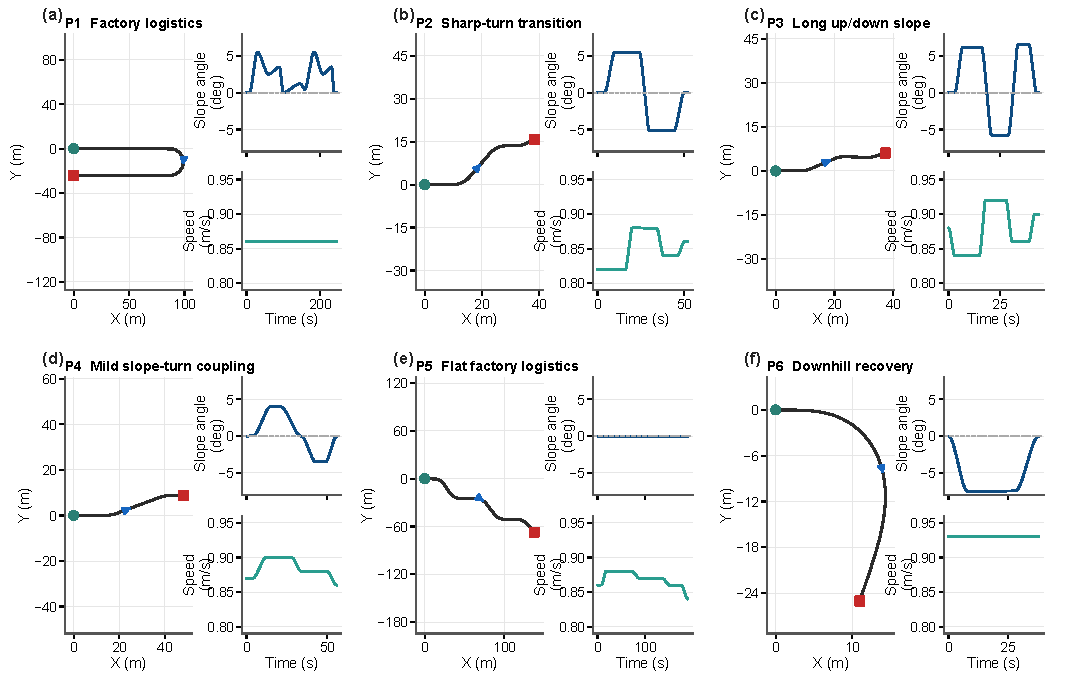
\includegraphics[width=\textwidth]{Fig03_Six_Route_Closed_Loop_Benchmark.pdf}
\caption{Six-route closed-loop benchmark. Each panel shows the complete planar reference path together with the aligned slope and reference-speed profiles. Green circles, red squares, and blue arrowheads mark route starts, route ends, and travel direction, respectively.}
\label{fig:closed_loop_route_set}
\end{figure*}

Model seed 42 was retained for the controller and fusion visualizations specified by those analyses. The four-estimator trace in Fig.~\ref{fig:representative_four_estimator_trace} uses seed 73 under a separate representativeness rule. Quantitative conclusions use all ten seeds and all six routes, while the representative traces illustrate runtime behavior alongside the complete summaries.

\subsection{Metrics and Statistical Analysis}

Offline primary metrics were slope-angle mean absolute error (MAE) and either the pre-specified $|\theta|\leq10^{\circ}$ P95 absolute error or the edge-region P95 absolute error, depending on the comparison. The frozen edge-region metric was the larger of the P95 absolute errors evaluated over $-10^{\circ}\leq\theta\leq-8^{\circ}$ and $8^{\circ}\leq\theta\leq10^{\circ}$. Closed-loop estimator accuracy was summarized by route-wise slope-angle MAE after the common 0.5-s warm-up and by the complete-trace P95 absolute error. The three inferential primary closed-loop outcomes were lateral-error RMS, heading-error RMS, and the composite input-increment index $J_{\Delta u}$. Lower values favor the target method. The composite input-increment index is defined as a control-regularity summary rather than a physical energy measure.

Paired effects are reported as comparator minus target so that positive values favor the target. Offline intervals resampled paired model seeds. Learned closed-loop intervals resampled model seeds first and then retained all six matched routes within each resampled seed; deterministic comparisons resampled routes. All reported bootstrap intervals used 10000 iterations and seed 20260715. Table~\ref{tab:evaluation_protocol} records the unit and interpretation of each evidence family.

\begin{table*}[!tbp]
\centering
\caption{\textbf{Evaluation metrics, statistical units, and interpretation rules.}}
\label{tab:evaluation_protocol}
\scriptsize
\setlength{\tabcolsep}{3pt}
\begin{tabular}{|p{0.19\textwidth}|p{0.25\textwidth}|p{0.16\textwidth}|p{0.16\textwidth}|p{0.16\textwidth}|}
\hline
Evidence family & Reported quantity & Unit & Statistical unit & Decision rule \\
\hline
Offline slope estimation & Slope-angle MAE; pre-specified P95 absolute error; edge-region P95 absolute error & deg & Ten paired model seeds & Positive comparator-minus-target effect favors target \\
Closed-loop slope estimation & Route-wise slope-angle MAE; complete-trace P95 absolute error & deg & Ten model seeds per route & Descriptive mean $\pm$ SD; lower values favor the method \\
Primary closed-loop inference & $e_y$ RMS; $e_\psi$ RMS; $J_{\Delta u}$ & m; rad; -- & Six paired routes or ten seeds $\times$ six routes & Route or hierarchical seed-first bootstrap \\
Fusion configuration & Fixed gain, innovation, NIS, correction, rate, and scheduling guards & -- & One locked interface configuration & Applied identically to all matched closed-loop cases \\
Fusion closed-loop comparison & $e_y$ RMS; $e_\psi$ RMS; $J_{\Delta u}$ & m; rad; -- & Ten seeds $\times$ six matched routes & Hierarchical seed-first paired bootstrap and matched mean reductions \\
Execution integrity & Case completion, constraint compliance, solver status, fallback identity, and runtime signal use & status & 60 matched cases & Checked independently of the performance aggregation \\
Estimator core runtime & p50, p95, p99, $>10$-ms count & ms & 10000 timed calls after 500 warm-ups & Compare methods only within the common ONNX Runtime CPU backend \\
\hline
\end{tabular}
\end{table*}

\subsection{Reproducibility and Reporting Boundaries}

The dataset, feature specification, model checkpoints, plant revision, six route definitions, LPV database, controller cache, metrics, thresholds, and seed set were fixed and identified by file checksums. A completeness check confirmed 40/40 offline estimator rows, 240/240 estimator closed-loop rows, 18/18 scheduling-necessity cases, and 60/60 matched fusion cases. A source cross-check covered the reported paired intervals and matched-case summaries without discrepancy.

\section{Results and Discussion}
\label{sec:results_discussion}

\subsection{Closed-Loop Performance Across Slope-Scheduling Conditions}
\label{subsec:slope_scheduling_conditions}

\begin{figure*}[!tbp]
\centering
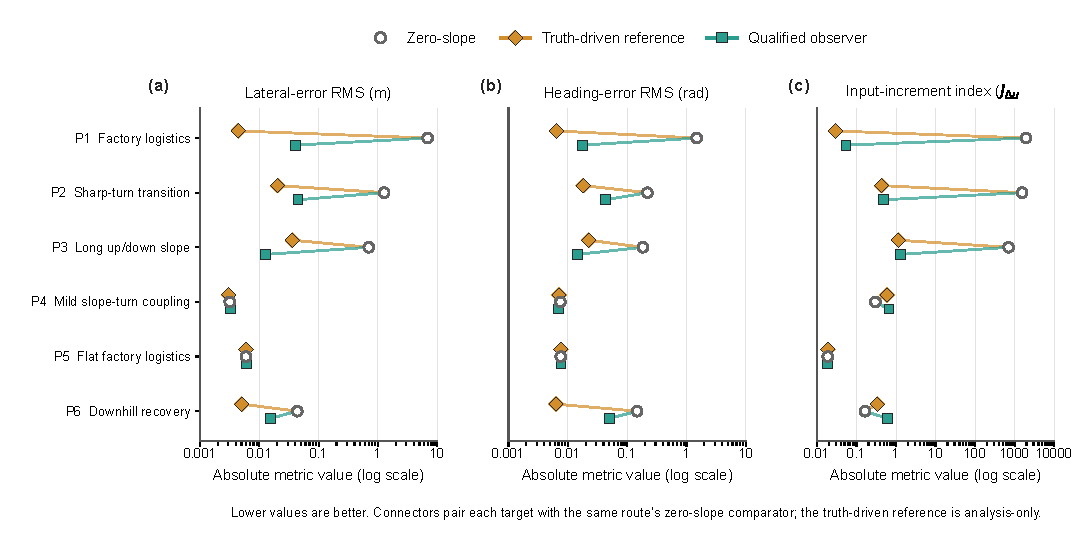
\includegraphics[width=\textwidth]{Fig04_Grade_Scheduling_Closed_Loop_Metrics.pdf}
\caption{Route-resolved absolute closed-loop metrics under zero-slope scheduling, the truth-driven conditioned reference, and qualified observer scheduling. Panels show (a) lateral-error RMS, (b) heading-error RMS, and (c) the composite input-increment index. White circles denote zero-slope scheduling, orange diamonds the truth-driven reference, and teal squares the qualified observer; connectors pair each slope-informed result with the same route's zero-slope comparator. Lower values indicate better performance, and logarithmic axes accommodate route-to-route scale differences. The truth-driven conditioned reference is analysis-only and represents an idealized scheduling reference rather than a deployable slope source.}
\label{fig:slope_necessity_effects}
\end{figure*}


Across the six routes, the absolute means followed the expected aggregate ordering from missing, through estimated, to exact slope information. Zero-slope scheduling yielded lateral-error RMS, heading-error RMS, and $J_{\Delta u}$ means of 1.48046~m, 0.34204~rad, and 696.014, respectively. The qualified observer reduced these values to 0.02051~m, 0.02347~rad, and 0.51646, while the analysis-only truth-driven reference yielded the lowest corresponding means of 0.01248~m, 0.01139~rad, and 0.42684. Relative to zero-slope scheduling, the mean reductions under the truth-driven reference were 1.46798~m, 0.33065~rad, and 695.587; the corresponding reductions under the qualified observer were 1.45995~m, 0.31857~rad, and 695.497. All six bootstrap confidence intervals reported in Table~\ref{tab:slope_necessity_effects} excluded zero. These aggregate results establish the control relevance of slope scheduling and indicate the additional performance potential provided by a more accurate scheduling signal.

\begin{table*}[!tbp]
\centering
\caption{\textbf{Six-route paired effects relative to zero-slope LPV-MPC. Effects are zero-slope minus target, so positive values favor the target. Boldface mean effects have 95\% confidence intervals excluding zero. The truth-driven conditioned reference is analysis-only.}}
\label{tab:slope_necessity_effects}
\setlength{\tabcolsep}{3pt}
\begin{tabular}{|l|l|r|r|r|}
\hline
Target source & Metric & Mean effect & 95\% CI & Routes \\
\hline
Truth-driven conditioned reference & $e_y$ RMS (m) & \textbf{1.46798} & [0.11715, 3.74682] & 6 \\
Truth-driven conditioned reference & $e_\psi$ RMS (rad) & \textbf{0.33065} & [0.05065, 0.80004] & 6 \\
Truth-driven conditioned reference & $J_{\Delta u}$ & \textbf{695.587} & [116.408, 1339.454] & 6 \\
Qualified observer & $e_y$ RMS (m) & \textbf{1.45995} & [0.11917, 3.72848] & 6 \\
Qualified observer & $e_\psi$ RMS (rad) & \textbf{0.31857} & [0.04460, 0.79161] & 6 \\
Qualified observer & $J_{\Delta u}$ & \textbf{695.497} & [116.277, 1339.412] & 6 \\
\hline
\end{tabular}
\end{table*}

The route-resolved results in Fig.~\ref{fig:slope_necessity_effects} support a clear aggregate hierarchy from missing, through estimated, to exact slope information. The truth-driven condition provides an analysis-only upper reference, whereas standalone scheduling with the qualified observer shows that a causal slope estimate recovers most of the closed-loop benefit. Section~\ref{subsec:slope_scheduling_conditions} therefore establishes that slope scheduling materially improves the LPV-MPC closed loop and that higher scheduling accuracy provides further performance potential. The standalone observer condition is included only to isolate the value of slope quality; the deployed fusion architecture is evaluated separately in Sections~\ref{subsec:bounded_fusion_runtime} and~\ref{subsec:fusion_closed_loop_comparison}. Table~\ref{tab:slope_necessity_effects} provides the corresponding paired effects and route-bootstrap confidence intervals.

\subsection{Offline Evaluation of the Multi-Scale Time-Lag Difference Representation}
\label{subsec:offline_delta_lag_evaluation}

\begin{figure*}[!tbp]
\centering
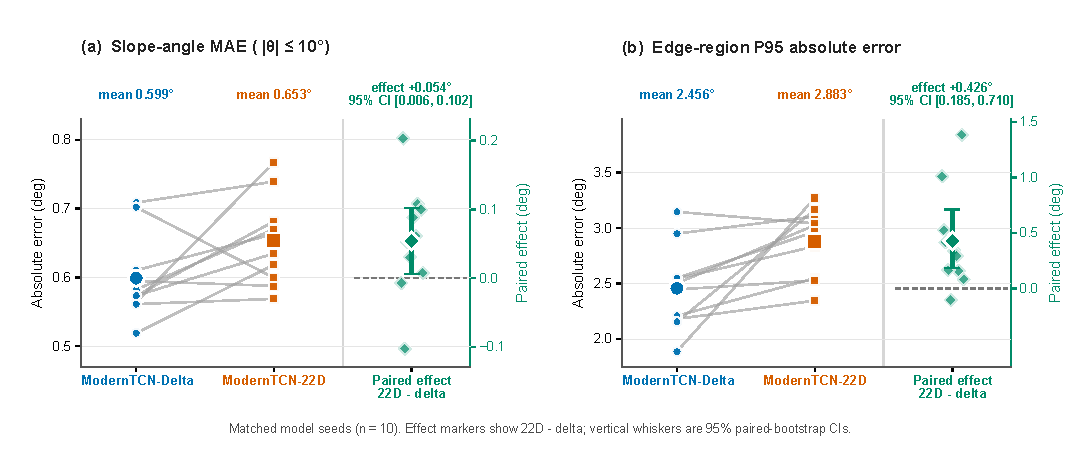
\includegraphics[width=\textwidth]{Fig05_Offline_Estimator_Comparison.pdf}
\caption{Matched-seed offline comparison of ModernTCN input representations. (a) Slope-angle MAE over test windows with $|\theta|\leq10^{\circ}$. (b) Edge-region P95 absolute slope-angle error. Blue circles and vermillion squares show individual results for ModernTCN-Delta and ModernTCN-22D, respectively; gray lines connect matched model seeds, and larger markers denote arithmetic means. Green diamonds show seed-paired effects defined as ModernTCN-22D minus ModernTCN-Delta. The larger diamond and vertical whiskers denote the mean effect and its 95\% paired-seed bootstrap confidence interval. Positive effects favor ModernTCN-Delta ($n=10$).}
\label{fig:offline_estimator_distribution}
\end{figure*}


Figure~\ref{fig:offline_estimator_distribution} isolates the effect of the multi-scale delta bank using ten matched model seeds. Over test windows with $|\theta|\leq10^{\circ}$, the mean slope-angle MAE decreased from 0.65300$^{\circ}$ for ModernTCN-22D to 0.59888$^{\circ}$ for ModernTCN-Delta. The paired effect was 0.05412$^{\circ}$ with a 95\% confidence interval of [0.00608, 0.10180]. In the edge region, the mean P95 absolute error decreased from 2.88256$^{\circ}$ to 2.45649$^{\circ}$, corresponding to a paired effect of 0.42608$^{\circ}$ [0.18517, 0.70987].

The broader four-estimator benchmark is reported in Table~\ref{tab:estimator_and_delta_results}. ModernTCN-Delta achieved the lowest mean MAE and pre-specified $|\theta|\leq10^{\circ}$ P95 absolute error, with supported paired advantages over GRU-22D and TCN-22D.

\begin{table*}[!tbp]
\centering
\caption{\textbf{Offline estimator comparison over ten matched model seeds. Panel A reports absolute means. Panel B reports comparator-minus-ModernTCN-Delta paired effects; positive effects favor ModernTCN-Delta, and boldface intervals exclude zero.}}
\label{tab:estimator_and_delta_results}
\scriptsize
\setlength{\tabcolsep}{2.6pt}
\begin{tabular}{|p{0.18\textwidth}|p{0.21\textwidth}|p{0.08\textwidth}|p{0.22\textwidth}|p{0.15\textwidth}|p{0.08\textwidth}|}
\hline
\multicolumn{6}{|l|}{\textit{Panel A: Absolute offline means}} \\
\hline
Method & MAE mean (deg) & MAE support & P95 mean (deg) & P95 region & P95 support \\
\hline
ModernTCN-Delta & 0.59888 & -- & 1.67777 & $|\theta|\leq10^{\circ}$ & -- \\
ModernTCN-22D & 0.65300 & -- & 1.80626 & $|\theta|\leq10^{\circ}$ & -- \\
GRU-22D & 0.88583 & -- & 2.25950 & $|\theta|\leq10^{\circ}$ & -- \\
TCN-22D & 0.91537 & -- & 2.63580 & $|\theta|\leq10^{\circ}$ & -- \\
\hline
\multicolumn{6}{|l|}{\textit{Panel B: Paired comparator-minus-ModernTCN-Delta effects}} \\
\hline
Comparator & MAE effect [95\% CI] (deg) & MAE support & P95 effect [95\% CI] (deg) & P95 region & P95 support \\
\hline
ModernTCN-22D & \textbf{0.05412 [0.00608, 0.10180]} & 8/10 & \textbf{0.42608 [0.18517, 0.70987]} & Edge region & 9/10 \\
GRU-22D & \textbf{0.28694 [0.18468, 0.37271]} & 9/10 & \textbf{0.58172 [0.38462, 0.80045]} & $|\theta|\leq10^{\circ}$ & 10/10 \\
TCN-22D & \textbf{0.31648 [0.24668, 0.38012]} & 10/10 & \textbf{0.95802 [0.69170, 1.25456]} & $|\theta|\leq10^{\circ}$ & 10/10 \\
\hline
\end{tabular}
\end{table*}

Figure~\ref{fig:offline_estimator_distribution} shows all ten matched seed pairs for the two ModernTCN input representations, while Table~\ref{tab:estimator_and_delta_results} retains the complete four-estimator comparison. Together, they identify ModernTCN-Delta as the strongest of the four tested configurations under the present evaluation protocol.

\subsection{Closed-Loop Accuracy of the Tested Slope Estimators}
\label{subsec:closed_loop_estimator_accuracy}

To determine whether the offline estimator ordering remained visible after deployment in the common simulation interface, the four-estimator closed-loop slope traces were compared. Figure~\ref{fig:representative_four_estimator_trace} shows the complete P2 Sharp-turn transition route. Model seed 73 was selected by a representativeness rule and ranked fourth among the ten P2 seeds by ModernTCN-Delta case-level MAE. The complete six-path, ten-seed summary is reported in Table~\ref{tab:closed_loop_estimator_accuracy}.

\begin{figure*}[!tbp]
\centering
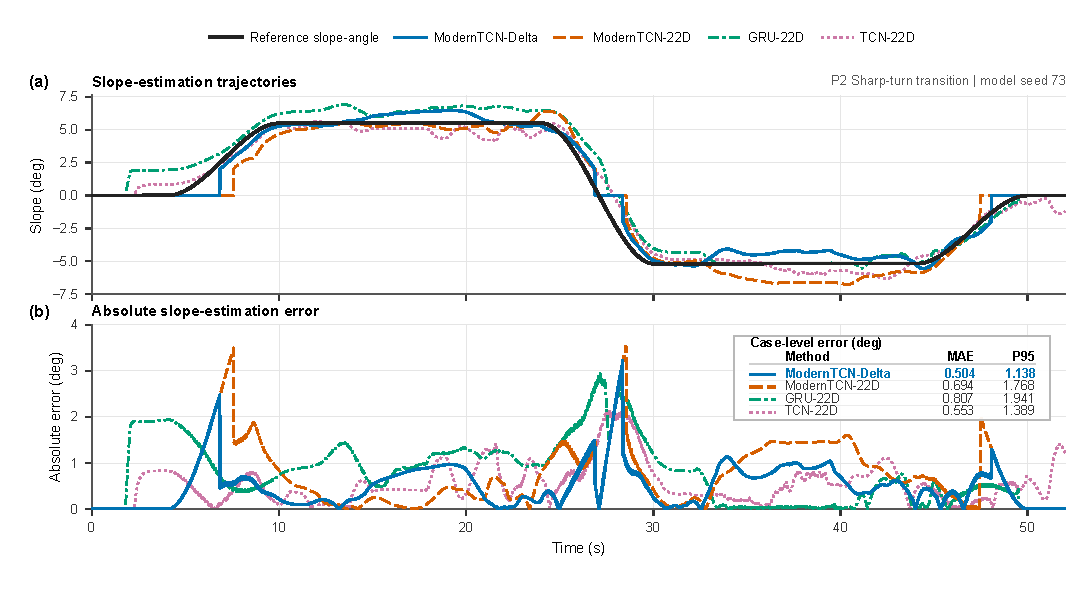
\includegraphics[width=\textwidth]{Fig06_Representative_Grade_Estimation_Traces.pdf}
\caption{\textbf{Representative closed-loop slope-estimation results on the P2 Sharp-turn transition route with model seed 73.} (a) Reference slope and estimates produced by ModernTCN-Delta, ModernTCN-22D, GRU-22D, and TCN-22D over the complete route. (b) Corresponding absolute slope-angle estimation errors. The inset reports case-level MAE after the common 0.5-s warm-up and complete-trace P95 absolute error. The displayed seed is a representative case selected independently of minimum error; the complete six-path, ten-seed results are reported in Table~\ref{tab:closed_loop_estimator_accuracy}.}
\label{fig:representative_four_estimator_trace}
\end{figure*}

In the displayed case, ModernTCN-Delta achieved the lowest MAE (0.504$^{\circ}$) and P95 absolute error (1.138$^{\circ}$), while the four trajectories reveal transition and steady-state characteristics beyond the offline distributions in Fig.~\ref{fig:offline_estimator_distribution}. Across the complete closed-loop benchmark, ModernTCN-Delta also had the lowest all-path mean MAE (0.423$^{\circ}$) and P95 absolute error (1.237$^{\circ}$). It ranked first on four of six routes for both metrics; ModernTCN-22D led P5, while GRU-22D and TCN-22D provided the lowest P3 MAE and P95, respectively.

\begin{table*}[!tbp]
\centering
\caption{\textbf{Path-wise closed-loop slope-estimation accuracy over ten matched model seeds.} Panel A reports slope-angle MAE after the common 0.5-s warm-up, and Panel B reports the complete-trace P95 absolute error. Entries are mean $\pm$ SD over ten seeds for each path. The All paths row first averages the six routes within each seed and then summarizes the ten seed-level means. Lower values indicate better performance; the best mean in each row is highlighted.}
\label{tab:closed_loop_estimator_accuracy}
\scriptsize
\setlength{\tabcolsep}{4.0pt}
{\renewcommand{\arraystretch}{1.08}
\begin{tabular}{@{}lcccc@{}}
\toprule
Path & ModernTCN-Delta & ModernTCN-22D & GRU-22D & TCN-22D \\
\midrule
\multicolumn{5}{@{}l}{\textit{Panel A: Slope-angle MAE (deg)}} \\
\addlinespace[1.5pt]
P1 Factory logistics & \textbf{0.458 $\pm$ 0.104} & 0.492 $\pm$ 0.156 & 0.827 $\pm$ 0.408 & 2.387 $\pm$ 0.833 \\
P2 Sharp-turn transition & \textbf{0.593 $\pm$ 0.107} & 0.645 $\pm$ 0.078 & 0.698 $\pm$ 0.197 & 0.783 $\pm$ 0.276 \\
P3 Long up/down slope & 0.791 $\pm$ 0.121 & 0.880 $\pm$ 0.087 & \textbf{0.763 $\pm$ 0.151} & 0.846 $\pm$ 0.232 \\
P4 Mild slope-turn coupling & \textbf{0.036 $\pm$ 0.062} & 0.037 $\pm$ 0.064 & 1.397 $\pm$ 0.451 & 1.237 $\pm$ 0.614 \\
P5 Flat factory logistics & 0.087 $\pm$ 0.223 & \textbf{0.046 $\pm$ 0.092} & 1.206 $\pm$ 0.750 & 1.249 $\pm$ 0.593 \\
P6 Downhill recovery & \textbf{0.570 $\pm$ 0.218} & 0.601 $\pm$ 0.193 & 0.746 $\pm$ 0.227 & 0.846 $\pm$ 0.517 \\
\textbf{All routes} & \textbf{0.423 $\pm$ 0.080} & 0.450 $\pm$ 0.046 & 0.940 $\pm$ 0.267 & 1.225 $\pm$ 0.434 \\
\midrule
\multicolumn{5}{@{}l}{\textit{Panel B: P95 absolute error (deg)}} \\
\addlinespace[1.5pt]
P1 Factory logistics & \textbf{1.434 $\pm$ 0.434} & 1.451 $\pm$ 0.613 & 2.528 $\pm$ 1.071 & 10.888 $\pm$ 4.279 \\
P2 Sharp-turn transition & \textbf{1.642 $\pm$ 0.299} & 1.847 $\pm$ 0.310 & 2.257 $\pm$ 0.558 & 1.850 $\pm$ 0.453 \\
P3 Long up/down slope & 2.289 $\pm$ 0.385 & 2.812 $\pm$ 0.407 & 2.270 $\pm$ 0.528 & \textbf{2.197 $\pm$ 0.495} \\
P4 Mild slope-turn coupling & \textbf{0.229 $\pm$ 0.723} & 0.244 $\pm$ 0.772 & 2.353 $\pm$ 0.732 & 1.469 $\pm$ 0.656 \\
P5 Flat factory logistics & 0.478 $\pm$ 1.024 & \textbf{0.455 $\pm$ 0.968} & 2.414 $\pm$ 0.641 & 1.512 $\pm$ 0.688 \\
P6 Downhill recovery & \textbf{1.351 $\pm$ 0.249} & 1.418 $\pm$ 0.291 & 1.792 $\pm$ 0.414 & 2.000 $\pm$ 0.643 \\
\textbf{All routes} & \textbf{1.237 $\pm$ 0.357} & 1.371 $\pm$ 0.316 & 2.269 $\pm$ 0.563 & 3.319 $\pm$ 1.014 \\
\bottomrule
\end{tabular}
}
\end{table*}

The offline and closed-loop estimator results therefore provide complementary evidence: Section~\ref{subsec:offline_delta_lag_evaluation} isolates the delta-bank representation under a common data protocol, whereas Section~\ref{subsec:closed_loop_estimator_accuracy} describes its behavior after integration into the closed-loop simulation. Controller-level benefit is evaluated separately in Section~\ref{subsec:fusion_closed_loop_comparison}, where the scheduling interface, route geometry, constrained optimizer, and command regularization determine how slope-estimation errors are translated into tracking metrics.

The final closed-loop MTCN-LPV-MPC benchmark achieved mean lateral-error RMS of 0.02635~m, heading-error RMS of 0.02216~rad, and $J_{\Delta u}=0.93053$ over six routes and ten model seeds. These values define the matched controller baseline used in Section~\ref{subsec:fusion_closed_loop_comparison}. The fusion comparison retains the same route--seed structure so that the effect of the bounded correction supplied by the qualified observer is evaluated directly rather than inferred from a separate deterministic source.

\subsection{Runtime Operation of the Bounded Fusion Interface}
\label{subsec:bounded_fusion_runtime}

The qualified observer uses the six-axis inertial configuration described in
Section~\ref{sec:adaptive_slope_fusion} and contributes through the bounded
correction channel. ModernTCN-Delta remains the primary slope source, while the
observer contributes when calibrated source uncertainty, estimated
helpfulness, and innovation consistency jointly support the correction. A
common set of activation, innovation-consistency, correction-amplitude, rate,
and scheduling guards was fixed for all matched cases, as summarized in
Table~\ref{tab:observer_fusion_evidence}. This design retains the learned
estimate as the nominal signal and conditions the observer contribution before
the fused slope enters the scheduling filter.

\begin{figure*}[!tbp]
\centering
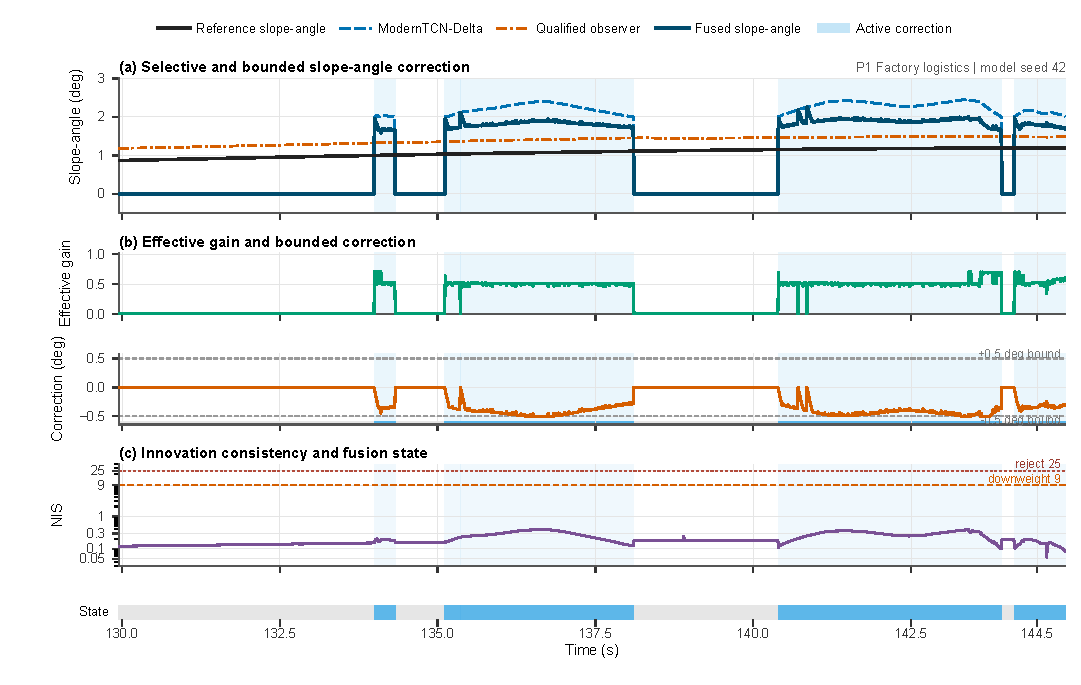
\includegraphics[width=\textwidth]{Fig07_Bounded_Fusion_Mechanism.pdf}
\caption{\textbf{Representative operation of the bounded fusion interface on the P1 Factory logistics route with model seed 42.} (a) Reference slope and the ModernTCN-Delta, qualified observer, and fused estimates. (b) Effective fusion gain and bounded slope correction. (c) Innovation consistency and active/fallback state. Shaded regions indicate active correction intervals. This representative case explains the runtime mechanism, while quantitative conclusions use all 60 matched route--seed pairs.}
\label{fig:fusion_mechanism_trace}
\end{figure*}

Figure~\ref{fig:fusion_mechanism_trace} illustrates how these conditions act
jointly at runtime. P1 was retained for the qualitative trace because it
contains slope variation, turning, and speed changes in one route, while model
seed 42 was specified a priori for qualitative visualization. Within this
case, the 129.95--144.94~s interval was chosen by a deterministic
maximum-active-fraction rule over fixed 15-s windows. The fused estimate
therefore coincides exactly with ModernTCN-Delta during fallback and receives a
limited observer correction in eligible intervals. This trace explains the
runtime mechanism, while quantitative inference uses all 60 matched
route--seed pairs.

The fixed interface was evaluated over all 60 matched route--seed cases, with
ground-truth slope excluded from the runtime fusion inputs. All cases completed
the prescribed constraint, solver, timeout, diagnostic, truth-access, and
fallback-identity checks. Table~\ref{tab:observer_fusion_evidence} summarizes
the configuration and execution checks, while Section~\ref{subsec:fusion_closed_loop_comparison} reports the paired
closed-loop performance effects.

\begin{table*}[!tbp]
\centering
\caption{\textbf{Fixed fusion configuration and execution summary. Figure~\ref{fig:fusion_mechanism_trace} shows the corresponding runtime behavior.}}
\label{tab:observer_fusion_evidence}
\scriptsize
\setlength{\tabcolsep}{3.2pt}
\begin{tabular}{|p{0.22\textwidth}|p{0.25\textwidth}|p{0.45\textwidth}|}
\hline
Component & Fixed value & Function in the deployed interface \\
\hline
Gain and activation
& $K_{\max}=1.0$; helpfulness 0.6; slope entry/exit $0.5^{\circ}/0.3^{\circ}$
& Activates a bounded observer correction while retaining ModernTCN-Delta as the primary source \\
Innovation consistency
& Minimum innovation $0.25^{\circ}$; gate $2^{\circ}$; NIS thresholds 9/25
& Suppresses weak or inconsistent corrections before slope scheduling \\
Correction dynamics
& Magnitude bound $0.5^{\circ}$; rate bound $5^{\circ}\,\mathrm{s}^{-1}$
& Limits the amplitude and temporal variation of the complementary update \\
Scheduling guard
& Deadband $1.3^{\circ}$; range $[-10^{\circ},10^{\circ}]$
& Produces the conditioned slope supplied consistently to LPV-MPC \\
Execution integrity
& 60/60 cases completed and passed the constraint, solver, timeout, diagnostic, and runtime truth-access checks
& Confirms consistent execution and exact fallback identity with ModernTCN-Delta \\
Evidence scope
& 10 model seeds $\times$ 6 routes; one locked interface configuration
& Supports mechanism and execution claims; paired performance effects are evaluated in Table~\ref{tab:five_source_closed_loop} \\
\hline
\end{tabular}
\end{table*}

\subsection{Closed-Loop Comparison of MTCN-LPV-MPC and Fusion-LPV-MPC}
\label{subsec:fusion_closed_loop_comparison}

Figure~\ref{fig:fusion_closed_loop_effects} and Table~\ref{tab:five_source_closed_loop}
jointly report the matched closed-loop comparison between MTCN-LPV-MPC and
Fusion-LPV-MPC. Figure~\ref{fig:fusion_closed_loop_effects} shows the complete
route--seed distribution and route-level heterogeneity, whereas
Table~\ref{tab:five_source_closed_loop} gives the aggregate means, relative
reductions, and paired bootstrap intervals. Across the 60 route--seed
pairs, the mean lateral-error RMS decreased from 0.02635~m to 0.01891~m,
corresponding to a 28.23\% reduction. The paired baseline-minus-fusion effect was
0.00744~m with a 95\% confidence interval of [0.00245, 0.01527]. The mean
heading-error RMS decreased from 0.02216~rad to 0.01933~rad, corresponding to
a 12.79\% reduction, with a paired effect of 0.00283~rad and a 95\% confidence
interval of [0.00064, 0.00615].

The composite input-increment index decreased from 0.93053 to 0.67361, giving
a 27.61\% reduction in the matched mean. Its paired effect was 0.25692, with a
95\% confidence interval of [$-0.01349$, 0.93333]. Together, the matched results
show interval-supported reductions in the two primary tracking measures and a
lower mean $J_{\Delta u}$. At the route-aggregated level, P1 Factory logistics
showed the clearest joint improvement, with lower mean lateral-error RMS,
heading-error RMS, and $J_{\Delta u}$ across the ten model seeds. The
route-level markers in Fig.~\ref{fig:fusion_closed_loop_effects} show the
complete dispersion of case-level effects around the aggregate improvements.

\begin{table*}[!tbp]
\centering
\caption{\textbf{Matched MTCN-LPV-MPC and Fusion-LPV-MPC results over 60 route--seed pairs. Effects are defined as MTCN-LPV-MPC minus Fusion-LPV-MPC; boldface intervals exclude zero.}}
\label{tab:five_source_closed_loop}
\scriptsize
\setlength{\tabcolsep}{4pt}
\begin{tabular}{|l|r|r|r|r|}
\hline
Metric & MTCN-LPV-MPC & Fusion-LPV-MPC & Relative reduction & Paired effect [95\% CI] \\
\hline
$e_y$ RMS (m)
& 0.02635 & 0.01891 & 28.23\%
& \textbf{0.00744 [0.00245, 0.01527]} \\
$e_\psi$ RMS (rad)
& 0.02216 & 0.01933 & 12.79\%
& \textbf{0.00283 [0.00064, 0.00615]} \\
$J_{\Delta u}$
& 0.93053 & 0.67361 & 27.61\%
& 0.25692 [$-0.01349$, 0.93333] \\
\hline
\end{tabular}
\end{table*}

\begin{figure*}[!tbp]
\centering
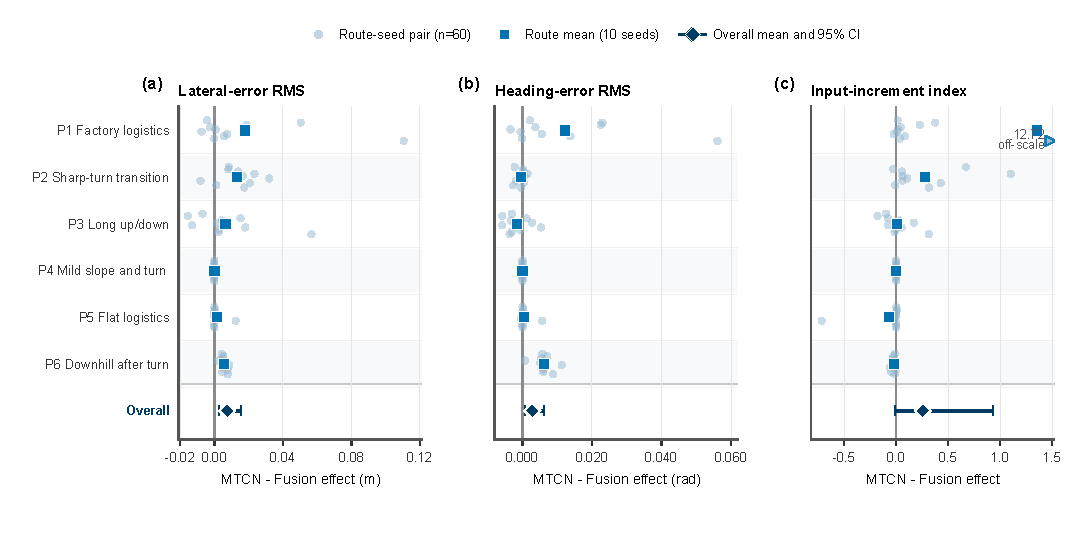
\includegraphics[width=\textwidth]{Fig08_Fusion_Closed_Loop_Effects.pdf}
\caption{\textbf{Matched closed-loop effects of the bounded fusion interface over 60 route--seed pairs.} Panels show MTCN-LPV-MPC minus Fusion-LPV-MPC effects for (a) lateral-error RMS, (b) heading-error RMS, and (c) the composite input-increment index. Light markers denote individual route--seed pairs, blue squares denote route-level means over ten seeds, and dark diamonds with whiskers denote the overall paired means with 95\% bootstrap confidence intervals. Positive effects favor Fusion-LPV-MPC. Exact ties remain at zero; the single distant $J_{\Delta u}$ case is labelled off-scale, while its overall interval is shown on the main axis. Aggregate values are reported in Table~\ref{tab:five_source_closed_loop}.}
\label{fig:fusion_closed_loop_effects}
\end{figure*}

This matched comparison isolates the incremental effect of the fusion
interface under the tested simulation conditions. The paired tracking
intervals support the complementary use of the qualified observer, while the
input-increment index summarizes the corresponding change in control
regularity. The bounded gain, correction limits, and exact fallback retain the
history-based estimate as the nominal control-facing source and leave command
generation in the model-based controller, consistent with hybrid
physics--learning designs
\citep{Hewing2020CautiousGPMPC,Zheng2024HybridPhysicsLearningUSV}.

\subsection{Estimator Inference Time and Model Size}
\label{subsec:estimator_inference_cost}

\begin{table*}[!tbp]
\centering
\caption{\textbf{Same-backend core inference time and model size for the four tested estimators. p50/p95/p99 denote latency percentiles over 10000 timed calls.}}
\label{tab:runtime_scope}
\scriptsize
\setlength{\tabcolsep}{3pt}
\begin{tabular}{|l|r|r|r|r|r|l|}
\hline
Method & Params (k) & Model (kB) & p50 (ms) & p95 (ms) & p99 (ms) & $>10$ ms \\
\hline
GRU-22D & 99.276 & 400.682 & 0.3071 & 0.3377 & 0.4124 & 0/10000 \\
ModernTCN-22D & 118.538 & 472.135 & 0.3582 & 0.3881 & 0.4942 & 0/10000 \\
ModernTCN-Delta & 145.202 & 578.793 & 0.3744 & 0.4038 & 0.4818 & 0/10000 \\
TCN-22D & 156.396 & 627.487 & 1.0452 & 1.1341 & 1.3597 & 1/10000 \\
\hline
\end{tabular}
\end{table*}


Under the common ONNX Runtime CPU backend, batch size one, one thread, 500 warm-ups, and 10000 timed calls, all four estimators had p95 core inference times below 1.2~ms (Table~\ref{tab:runtime_scope}). ModernTCN-Delta achieved a p95 of 0.4038~ms with no call above 10~ms. GRU-22D was the fastest core predictor, while TCN-22D produced one call above 10~ms. The sub-millisecond cores leave substantial margin within the 10-ms control period without requiring solver-side acceleration of the kind pursued by parallel NMPC implementations \citep{Xu2024ParallelNMPC}. These same-backend measurements characterize estimator inference only and are not used to rank unmeasured wrappers or controller interfaces.

\subsection{Integrated Discussion and Scope}
\label{subsec:integrated_discussion_scope}

Taken together, the experiments establish a staged perception-to-control relationship. The truth-driven comparison first shows that slope is a consequential scheduling variable for the LPV-MPC with fixed tuning. ModernTCN-Delta then improves slope estimation under the common offline protocol and retains the lowest all-path mean MAE and P95 error after deployment in the closed-loop simulation interface. These estimator-level results support slope-source selection, while controller performance is evaluated separately because scheduling, route geometry, constraints, and command regularization transform estimation errors before they appear in closed-loop metrics.

The qualified observer complements the learned history-based estimate through
an inertial error structure admitted by the calibrated,
innovation-conditioned correction channel. Across the matched closed-loop
cases, this arrangement reduced lateral-error RMS by 28.23\%, heading-error
RMS by 12.79\%, and the mean input-increment index by 27.61\%. The paired
confidence intervals support the reductions in the two tracking measures,
while all three matched means favor the fused configuration. Because the
temporal estimate remains the primary source and every correction
is bounded before scheduling, the fusion gain is obtained without transferring
command generation to the learning or observer blocks. The resulting structure aligns
with prior use of model-based information to manage slope-estimation
uncertainty \citep{Liu2023RoadSlopeAAIMM,Gao2024RoadSlopeHDV,Feng2021MultiModelFusion} and with hybrid
physics--learning designs that retain the model-based controller as the
command-generating mechanism \citep{Zheng2024HybridPhysicsLearningUSV}.

\FloatBarrier
\section{Conclusion}
\label{sec:conclusion}

This study developed a slope-aware perception-to-control framework for a
diagonal dual-steering-wheel AGV. The framework combines history-based slope
estimation, a bounded correction supplied by the qualified observer, and
synchronized slope scheduling within LPV-MPC. ModernTCN-Delta estimates road
slope from historical AGV responses without requiring a direct slope
measurement, while the conditioned slope signal is consistently incorporated
into the prediction model, measured-disturbance channel, slope feedforward,
scheduled weights, and constraints.

The experimental results confirm the control relevance of slope scheduling.
Compared with zero-slope scheduling, causal slope information substantially
improved closed-loop tracking and the input-increment measure, while the
analysis-only truth-driven condition indicated further performance potential
from increased scheduling accuracy. The multi-scale time-lag difference representation
improved offline slope estimation, and ModernTCN-Delta achieved the strongest
overall accuracy among the tested estimators. This advantage was retained after
deployment in the common closed-loop simulation interface. The same-backend
inference measurements further indicate that the estimator cores are compatible
with the control period under the tested CPU configuration.

The bounded fusion interface complemented the history-based estimate through
calibrated, innovation-conditioned, and amplitude-limited observer corrections.
In the matched closed-loop comparison, Fusion-LPV-MPC produced supported
reductions in both lateral- and heading-tracking errors relative to
MTCN-LPV-MPC, together with a lower mean input-increment index. The prescribed
execution checks also confirmed bounded correction, exact fallback to
ModernTCN-Delta, and the exclusion of ground-truth slope from the runtime fusion
inputs. These results show that complementary physics-based information can
improve slope-aware control while retaining the learned estimator as the
primary slope source and the model-based controller as the command-generating
mechanism.

Future work will extend the present simulation evidence through
hardware-in-the-loop and physical-vehicle experiments under broader route,
load, speed, and measurement-disturbance conditions. Further research will also
address systematic parameter calibration and formal stability and error-bound
analysis for the slope-scheduled LPV-MPC framework.

\bibliographystyle{IEEEtran}
\bibliography{References}




% Keep the three author biographies together in the right column of the final page.
\makeatletter
\def\@IEEEBIOskipN{1.25\baselineskip}
\makeatother
\newpage

\begin{IEEEbiography}[{
\includegraphics[width=1in,height=1.25in,clip,keepaspectratio]{zpf.png}}]{Pengfei Zhang} was born in Heilongjiang, China. He received the B.S. and Ph.D. degrees from Dalian Maritime University. His current research interests include stabilization/tracking control of underactuated surface/underwater vehicles, nonlinear systems, and disturbance observers. He is currently working at Huzhou Normal University.
\end{IEEEbiography}

\begin{IEEEbiography}[{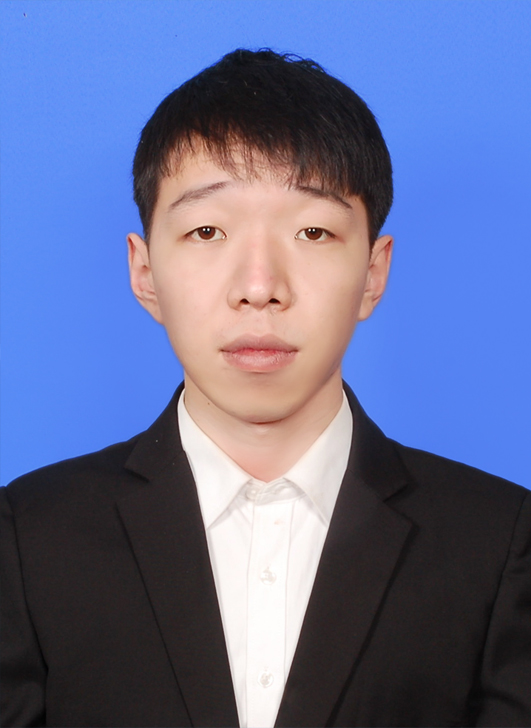
\includegraphics[width=1in,height=1.25in,clip,keepaspectratio]{tyh.png}}]{Yuhang Tang} received the B.Eng. degree in electrical engineering and automation from Shenyang Institute of Engineering, Shenyang, China, in 2019. He is currently pursuing the M.Eng. at Huzhou Normal University, Huzhou, China. His research interests include automated guided vehicle (AGV) control, autonomous navigation and path planning, deep learning, and intelligent robotic systems.
\end{IEEEbiography}

\begin{IEEEbiography}[{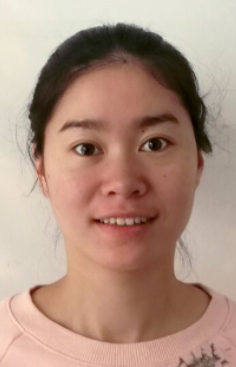
\includegraphics[width=1in,height=1.25in,clip,keepaspectratio]{ytt.png}}]{Tingting Yang} received the B.S. and Ph.D. degrees from Dalian Maritime University. Her current research interests include the formation control of autonomous vehicles, disturbance observers, and fault tolerant control. She is currently working at Huzhou Normal University.
\end{IEEEbiography}

\vskip 0pt plus 1filll\relax









\EOD

\end{document}
